% Options for packages loaded elsewhere
\PassOptionsToPackage{unicode}{hyperref}
\PassOptionsToPackage{hyphens}{url}
\documentclass[
  10pt,
]{article}
\usepackage{xcolor}
\usepackage[margin=0.82in]{geometry}
\usepackage{amsmath,amssymb}
\setcounter{secnumdepth}{5}
\usepackage{iftex}
\ifPDFTeX
  \usepackage[T1]{fontenc}
  \usepackage[utf8]{inputenc}
  \usepackage{textcomp} % provide euro and other symbols
\else % if luatex or xetex
  \usepackage{unicode-math} % this also loads fontspec
  \defaultfontfeatures{Scale=MatchLowercase}
  \defaultfontfeatures[\rmfamily]{Ligatures=TeX,Scale=1}
\fi
\usepackage{lmodern}
\ifPDFTeX\else
  % xetex/luatex font selection
\fi
% Use upquote if available, for straight quotes in verbatim environments
\IfFileExists{upquote.sty}{\usepackage{upquote}}{}
\IfFileExists{microtype.sty}{% use microtype if available
  \usepackage[]{microtype}
  \UseMicrotypeSet[protrusion]{basicmath} % disable protrusion for tt fonts
}{}
\makeatletter
\@ifundefined{KOMAClassName}{% if non-KOMA class
  \IfFileExists{parskip.sty}{%
    \usepackage{parskip}
  }{% else
    \setlength{\parindent}{0pt}
    \setlength{\parskip}{6pt plus 2pt minus 1pt}}
}{% if KOMA class
  \KOMAoptions{parskip=half}}
\makeatother
\usepackage{color}
\usepackage{fancyvrb}
\newcommand{\VerbBar}{|}
\newcommand{\VERB}{\Verb[commandchars=\\\{\}]}
\DefineVerbatimEnvironment{Highlighting}{Verbatim}{commandchars=\\\{\}}
% Add ',fontsize=\small' for more characters per line
\usepackage{framed}
\definecolor{shadecolor}{RGB}{248,248,248}
\newenvironment{Shaded}{\begin{snugshade}}{\end{snugshade}}
\newcommand{\AlertTok}[1]{\textcolor[rgb]{0.94,0.16,0.16}{#1}}
\newcommand{\AnnotationTok}[1]{\textcolor[rgb]{0.56,0.35,0.01}{\textbf{\textit{#1}}}}
\newcommand{\AttributeTok}[1]{\textcolor[rgb]{0.13,0.29,0.53}{#1}}
\newcommand{\BaseNTok}[1]{\textcolor[rgb]{0.00,0.00,0.81}{#1}}
\newcommand{\BuiltInTok}[1]{#1}
\newcommand{\CharTok}[1]{\textcolor[rgb]{0.31,0.60,0.02}{#1}}
\newcommand{\CommentTok}[1]{\textcolor[rgb]{0.56,0.35,0.01}{\textit{#1}}}
\newcommand{\CommentVarTok}[1]{\textcolor[rgb]{0.56,0.35,0.01}{\textbf{\textit{#1}}}}
\newcommand{\ConstantTok}[1]{\textcolor[rgb]{0.56,0.35,0.01}{#1}}
\newcommand{\ControlFlowTok}[1]{\textcolor[rgb]{0.13,0.29,0.53}{\textbf{#1}}}
\newcommand{\DataTypeTok}[1]{\textcolor[rgb]{0.13,0.29,0.53}{#1}}
\newcommand{\DecValTok}[1]{\textcolor[rgb]{0.00,0.00,0.81}{#1}}
\newcommand{\DocumentationTok}[1]{\textcolor[rgb]{0.56,0.35,0.01}{\textbf{\textit{#1}}}}
\newcommand{\ErrorTok}[1]{\textcolor[rgb]{0.64,0.00,0.00}{\textbf{#1}}}
\newcommand{\ExtensionTok}[1]{#1}
\newcommand{\FloatTok}[1]{\textcolor[rgb]{0.00,0.00,0.81}{#1}}
\newcommand{\FunctionTok}[1]{\textcolor[rgb]{0.13,0.29,0.53}{\textbf{#1}}}
\newcommand{\ImportTok}[1]{#1}
\newcommand{\InformationTok}[1]{\textcolor[rgb]{0.56,0.35,0.01}{\textbf{\textit{#1}}}}
\newcommand{\KeywordTok}[1]{\textcolor[rgb]{0.13,0.29,0.53}{\textbf{#1}}}
\newcommand{\NormalTok}[1]{#1}
\newcommand{\OperatorTok}[1]{\textcolor[rgb]{0.81,0.36,0.00}{\textbf{#1}}}
\newcommand{\OtherTok}[1]{\textcolor[rgb]{0.56,0.35,0.01}{#1}}
\newcommand{\PreprocessorTok}[1]{\textcolor[rgb]{0.56,0.35,0.01}{\textit{#1}}}
\newcommand{\RegionMarkerTok}[1]{#1}
\newcommand{\SpecialCharTok}[1]{\textcolor[rgb]{0.81,0.36,0.00}{\textbf{#1}}}
\newcommand{\SpecialStringTok}[1]{\textcolor[rgb]{0.31,0.60,0.02}{#1}}
\newcommand{\StringTok}[1]{\textcolor[rgb]{0.31,0.60,0.02}{#1}}
\newcommand{\VariableTok}[1]{\textcolor[rgb]{0.00,0.00,0.00}{#1}}
\newcommand{\VerbatimStringTok}[1]{\textcolor[rgb]{0.31,0.60,0.02}{#1}}
\newcommand{\WarningTok}[1]{\textcolor[rgb]{0.56,0.35,0.01}{\textbf{\textit{#1}}}}
\usepackage{graphicx}
\makeatletter
\newsavebox\pandoc@box
\newcommand*\pandocbounded[1]{% scales image to fit in text height/width
  \sbox\pandoc@box{#1}%
  \Gscale@div\@tempa{\textheight}{\dimexpr\ht\pandoc@box+\dp\pandoc@box\relax}%
  \Gscale@div\@tempb{\linewidth}{\wd\pandoc@box}%
  \ifdim\@tempb\p@<\@tempa\p@\let\@tempa\@tempb\fi% select the smaller of both
  \ifdim\@tempa\p@<\p@\scalebox{\@tempa}{\usebox\pandoc@box}%
  \else\usebox{\pandoc@box}%
  \fi%
}
% Set default figure placement to htbp
\def\fps@figure{htbp}
\makeatother
\setlength{\emergencystretch}{3em} % prevent overfull lines
\providecommand{\tightlist}{%
  \setlength{\itemsep}{0pt}\setlength{\parskip}{0pt}}
\usepackage{booktabs}
\usepackage{float}
\usepackage{xcolor}
\setcounter{tocdepth}{1}
\setlength{\parindent}{0pt}
\setlength{\parskip}{0.25em}
\usepackage{bookmark}
\IfFileExists{xurl.sty}{\usepackage{xurl}}{} % add URL line breaks if available
\urlstyle{same}
\hypersetup{
  hidelinks,
  pdfcreator={LaTeX via pandoc}}

\author{}
\date{\vspace{-2.5em}}

\begin{document}

\begin{center}
\IfFileExists{report_assets/upc_logo.png}{
\includegraphics[width=0.20\textwidth]{report_assets/upc_logo.png}\\[0.45em]}{}
{\LARGE\bfseries PCA Report}\\[0.45em]
Student name: Van Thinh TO\\
Student ID: 22518830\\[0.35em]
\end{center}

\vspace{1em}
\vspace{1em}
\tableofcontents
\newpage

\section{Set up}\label{set-up}

\begin{Shaded}
\begin{Highlighting}[]
\NormalTok{knitr}\SpecialCharTok{::}\NormalTok{opts\_chunk}\SpecialCharTok{$}\FunctionTok{set}\NormalTok{(}
  \AttributeTok{echo =} \ConstantTok{TRUE}\NormalTok{, }\AttributeTok{message =} \ConstantTok{FALSE}\NormalTok{, }\AttributeTok{warning =} \ConstantTok{FALSE}\NormalTok{,}
  \AttributeTok{fig.align =} \StringTok{"center"}\NormalTok{, }\AttributeTok{fig.pos =} \StringTok{"H"}\NormalTok{,}
  \AttributeTok{out.width =} \StringTok{"72\%"}\NormalTok{, }\AttributeTok{dpi =} \DecValTok{200}\NormalTok{, }\AttributeTok{dev =} \StringTok{"pdf"}\NormalTok{, }\AttributeTok{comment =} \StringTok{"\#\#"}
\NormalTok{)}

\FunctionTok{options}\NormalTok{(}\AttributeTok{digits =} \DecValTok{4}\NormalTok{)}

\FunctionTok{library}\NormalTok{(FactoMineR)}
\FunctionTok{library}\NormalTok{(cluster)}
\FunctionTok{library}\NormalTok{(fpc)}
\FunctionTok{library}\NormalTok{(pheatmap)}

\NormalTok{shape\_names }\OtherTok{\textless{}{-}} \FunctionTok{c}\NormalTok{(}\StringTok{"rEV21"}\NormalTok{, }\StringTok{"rEV32"}\NormalTok{, }\StringTok{"rEV31"}\NormalTok{)}
\NormalTok{five\_names }\OtherTok{\textless{}{-}} \FunctionTok{c}\NormalTok{(shape\_names, }\StringTok{"Num\_Atoms"}\NormalTok{, }\StringTok{"Rg"}\NormalTok{)}
\NormalTok{cluster\_colors }\OtherTok{\textless{}{-}} \FunctionTok{c}\NormalTok{(}\StringTok{"\#2C7FB8"}\NormalTok{, }\StringTok{"\#D95F02"}\NormalTok{, }\StringTok{"\#33A02C"}\NormalTok{, }\StringTok{"\#8C1D40"}\NormalTok{)}
\NormalTok{origin\_colors }\OtherTok{\textless{}{-}} \FunctionTok{c}\NormalTok{(}\AttributeTok{PROT =} \StringTok{"\#2C7FB8"}\NormalTok{, }\AttributeTok{RNA =} \StringTok{"\#8C1D40"}\NormalTok{)}
\end{Highlighting}
\end{Shaded}

\section{Session 1 --- PCA}\label{session-1-pca}

PCA combines measurements into new axes. PC1 captures the most
variation; PC2 captures the most remaining variation in a perpendicular
direction. \textbf{Variance} measures spread between pockets.
\textbf{Scores} are their coordinates on these axes. PCA centers the
measurements automatically; scaling also divides them by their standard
deviations (SDs).

\subsection{Import and check the data}\label{import-and-check-the-data}

We inspect column types, missing values, and Origin counts before
analysis.

\begin{Shaded}
\begin{Highlighting}[]
\CommentTok{\# Read the file and show a short preview of each column.}
\NormalTok{d1 }\OtherTok{\textless{}{-}} \FunctionTok{read.csv}\NormalTok{(}\StringTok{"data\_NS.csv"}\NormalTok{, }\AttributeTok{stringsAsFactors =} \ConstantTok{TRUE}\NormalTok{)}
\FunctionTok{str}\NormalTok{(d1, }\AttributeTok{vec.len =} \DecValTok{2}\NormalTok{, }\AttributeTok{strict.width =} \StringTok{"cut"}\NormalTok{, }\AttributeTok{width =} \DecValTok{75}\NormalTok{)}
\end{Highlighting}
\end{Shaded}

\begin{verbatim}
## 'data.frame':    600 obs. of  10 variables:
##  $ PDB_ID   : Factor w/ 600 levels "ID_001","ID_002",..: 498 464 504 303 ..
##  $ Origin   : Factor w/ 2 levels "PROT","RNA": 1 1 1 1 1 ...
##  $ Pocket   : Factor w/ 564 levels "0DU_4000-B","0EC_101-A",..: 7 347 192..
##  $ Eigval.1 : num  28.7 31.9 ...
##  $ Eigval.2 : num  20.3 15.6 ...
##  $ Eigval.3 : num  10.3 11 ...
##  $ rEV21    : num  0.709 0.49 ...
##  $ rEV32    : num  0.508 0.705 ...
##  $ rEV31    : num  0.36 0.345 ...
##  $ Num_Atoms: int  135 117 160 180 132 ...
\end{verbatim}

\begin{Shaded}
\begin{Highlighting}[]
\CommentTok{\# Count missing entries and pockets of each Origin.}
\FunctionTok{colSums}\NormalTok{(}\FunctionTok{is.na}\NormalTok{(d1))}
\end{Highlighting}
\end{Shaded}

\begin{verbatim}
##    PDB_ID    Origin    Pocket  Eigval.1  Eigval.2  Eigval.3     rEV21     rEV32 
##         0         0         0         0         0         0         0         0 
##     rEV31 Num_Atoms 
##         0         0
\end{verbatim}

\begin{Shaded}
\begin{Highlighting}[]
\FunctionTok{table}\NormalTok{(d1}\SpecialCharTok{$}\NormalTok{Origin)}
\end{Highlighting}
\end{Shaded}

\begin{verbatim}
## 
## PROT  RNA 
##  300  300
\end{verbatim}

\textbf{Reading the data:} \texttt{PDB\_ID} and \texttt{Pocket} are
identifiers; \texttt{Origin} is RNA or protein. \texttt{Eigval.1},
\texttt{.2}, and \texttt{.3} describe atomic spread along the largest,
intermediate, and smallest pocket axes. The ratios are
\(rEV21=\lambda_2/\lambda_1\), \(rEV32=\lambda_3/\lambda_2\), and
\(rEV31=\lambda_3/\lambda_1\); they describe shape proportions.
\texttt{Num\_Atoms} counts atoms and describes size. The missing-value
output gives one count per column; the Origin output gives group counts.

\textbf{Answer:} There are 600 pockets, 10 columns, 300 RNA and 300
protein pockets, and no missing values. Identifiers are excluded from
PCA.

\subsection{Shape-only PCA, without
scaling}\label{shape-only-pca-without-scaling}

We use the three ratios to study shape alone.
\texttt{scale.unit\ =\ FALSE} keeps their original scales.
\texttt{quali.sup\ =\ 4} makes the fourth column, \texttt{Origin},
supplementary: it labels groups without determining the axes.

\begin{Shaded}
\begin{Highlighting}[]
\CommentTok{\# Calculate PCA from the three shape ratios only.}
\NormalTok{shape\_input }\OtherTok{\textless{}{-}}\NormalTok{ d1[}\FunctionTok{c}\NormalTok{(shape\_names, }\StringTok{"Origin"}\NormalTok{)]}
\NormalTok{pca1 }\OtherTok{\textless{}{-}} \FunctionTok{PCA}\NormalTok{(shape\_input, }\AttributeTok{scale.unit =} \ConstantTok{FALSE}\NormalTok{, }\AttributeTok{quali.sup =} \DecValTok{4}\NormalTok{, }\AttributeTok{graph =} \ConstantTok{FALSE}\NormalTok{)}
\NormalTok{pca1}\SpecialCharTok{$}\NormalTok{eig}
\end{Highlighting}
\end{Shaded}

\begin{verbatim}
##        eigenvalue percentage of variance cumulative percentage of variance
## comp 1  0.0486643                59.7435                             59.74
## comp 2  0.0321893                39.5177                             99.26
## comp 3  0.0006018                 0.7389                            100.00
\end{verbatim}

\textbf{Table columns:} \texttt{eigenvalue} is the variance captured by
that PC; \texttt{percentage\ of\ variance} is its share of the total;
\texttt{cumulative\ percentage} adds the shares from PC1 through that
row. These PCA eigenvalues describe variation across pockets, unlike the
geometric eigenvalues in the CSV.

\begin{Shaded}
\begin{Highlighting}[]
\CommentTok{\# Plot pockets, colored by Origin; nearby points have similar shape scores.}
\FunctionTok{plot}\NormalTok{(pca1, }\AttributeTok{choix =} \StringTok{"ind"}\NormalTok{, }\AttributeTok{habillage =} \DecValTok{4}\NormalTok{, }\AttributeTok{label =} \StringTok{"none"}\NormalTok{,}
     \AttributeTok{title =} \StringTok{"Shape PCA: Origin"}\NormalTok{)}
\end{Highlighting}
\end{Shaded}

\begin{figure}[H]

{\centering 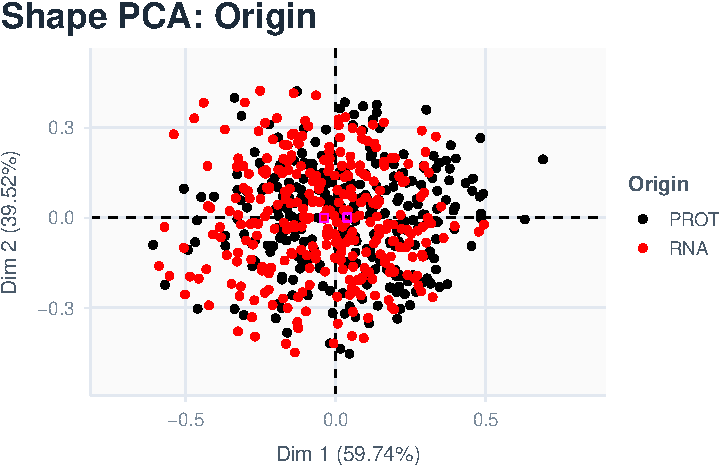
\includegraphics[width=0.72\linewidth]{pca_report_files/figure-latex/shape-plane-1} 

}

\caption{Shape-only PCA with supplementary Origin.}\label{fig:shape-plane}
\end{figure}

We check redundancy numerically rather than relying on the PCA alone.

\begin{Shaded}
\begin{Highlighting}[]
\CommentTok{\# Compare ratios and test whether the third is the product of the first two.}
\NormalTok{shape\_cor }\OtherTok{\textless{}{-}} \FunctionTok{cor}\NormalTok{(d1[shape\_names])}
\NormalTok{shape\_cor}
\end{Highlighting}
\end{Shaded}

\begin{verbatim}
##          rEV21    rEV32  rEV31
## rEV21  1.00000 -0.06497 0.6126
## rEV32 -0.06497  1.00000 0.7158
## rEV31  0.61255  0.71583 1.0000
\end{verbatim}

\begin{Shaded}
\begin{Highlighting}[]
\NormalTok{redundancy\_error }\OtherTok{\textless{}{-}} \FunctionTok{max}\NormalTok{(}\FunctionTok{abs}\NormalTok{(d1}\SpecialCharTok{$}\NormalTok{rEV31 }\SpecialCharTok{{-}}\NormalTok{ d1}\SpecialCharTok{$}\NormalTok{rEV21 }\SpecialCharTok{*}\NormalTok{ d1}\SpecialCharTok{$}\NormalTok{rEV32))}
\NormalTok{redundancy\_error}
\end{Highlighting}
\end{Shaded}

\begin{verbatim}
## [1] 0.0001051
\end{verbatim}

\textbf{Correlation table:} Rows and columns identify measurements.
Their intersection ranges from -1 to +1: positive means increasing
together, negative means moving oppositely, and near zero means little
linear relation. The diagonal is 1; the two halves repeat the same
comparisons.

\textbf{Answer:} PC3 captures only 0.74\%; the first two PCs retain
99.26\%. The ratios repeat information because
\(rEV31=rEV21\times rEV32\), with maximum discrepancy 1.05e-04,
consistent with rounding. PC3 is not exactly zero because this relation
is multiplicative, while PCA captures linear variation. RNA and protein
points overlap widely; shape does not clearly separate Origins.

\subsection{Add size and compare
scaling}\label{add-size-and-compare-scaling}

We compute \(Rg=\sqrt{Eigval1+Eigval2+Eigval3}\), which measures atomic
spread around the pocket center. We then use the same five measurements
in two PCAs, changing only scaling to identify its effect.

\begin{Shaded}
\begin{Highlighting}[]
\CommentTok{\# Add Rg and run the five{-}variable PCA before and after scaling.}
\NormalTok{d1}\SpecialCharTok{$}\NormalTok{Rg }\OtherTok{\textless{}{-}} \FunctionTok{sqrt}\NormalTok{(d1}\SpecialCharTok{$}\NormalTok{Eigval}\FloatTok{.1} \SpecialCharTok{+}\NormalTok{ d1}\SpecialCharTok{$}\NormalTok{Eigval}\FloatTok{.2} \SpecialCharTok{+}\NormalTok{ d1}\SpecialCharTok{$}\NormalTok{Eigval}\FloatTok{.3}\NormalTok{)}
\NormalTok{five\_input }\OtherTok{\textless{}{-}}\NormalTok{ d1[}\FunctionTok{c}\NormalTok{(five\_names, }\StringTok{"Origin"}\NormalTok{)]}
\NormalTok{pca\_raw }\OtherTok{\textless{}{-}} \FunctionTok{PCA}\NormalTok{(five\_input, }\AttributeTok{scale.unit =} \ConstantTok{FALSE}\NormalTok{, }\AttributeTok{quali.sup =} \DecValTok{6}\NormalTok{, }\AttributeTok{graph =} \ConstantTok{FALSE}\NormalTok{)}
\NormalTok{pca2 }\OtherTok{\textless{}{-}} \FunctionTok{PCA}\NormalTok{(five\_input, }\AttributeTok{scale.unit =} \ConstantTok{TRUE}\NormalTok{, }\AttributeTok{quali.sup =} \DecValTok{6}\NormalTok{, }\AttributeTok{graph =} \ConstantTok{FALSE}\NormalTok{)}

\CommentTok{\# Check how much raw variance each measurement contributes.}
\NormalTok{raw\_variance }\OtherTok{\textless{}{-}} \FunctionTok{numeric}\NormalTok{(}\DecValTok{5}\NormalTok{)}
\FunctionTok{names}\NormalTok{(raw\_variance) }\OtherTok{\textless{}{-}}\NormalTok{ five\_names}
\ControlFlowTok{for}\NormalTok{ (i }\ControlFlowTok{in} \DecValTok{1}\SpecialCharTok{:}\DecValTok{5}\NormalTok{) \{}
\NormalTok{  raw\_variance[i] }\OtherTok{\textless{}{-}} \FunctionTok{var}\NormalTok{(d1[[five\_names[i]]])}
\NormalTok{\}}
\FunctionTok{data.frame}\NormalTok{(}\AttributeTok{Variable =}\NormalTok{ five\_names, }\AttributeTok{Variance =}\NormalTok{ raw\_variance,}
           \AttributeTok{Percent =} \DecValTok{100} \SpecialCharTok{*}\NormalTok{ raw\_variance }\SpecialCharTok{/} \FunctionTok{sum}\NormalTok{(raw\_variance))}
\end{Highlighting}
\end{Shaded}

\begin{verbatim}
##            Variable  Variance   Percent
## rEV21         rEV21 2.842e-02 4.057e-04
## rEV32         rEV32 3.402e-02 4.857e-04
## rEV31         rEV31 1.915e-02 2.733e-04
## Num_Atoms Num_Atoms 7.004e+03 9.998e+01
## Rg               Rg 1.472e+00 2.101e-02
\end{verbatim}

\begin{Shaded}
\begin{Highlighting}[]
\CommentTok{\# Compare the individual PCs\textquotesingle{} explained{-}variance percentages.}
\FunctionTok{data.frame}\NormalTok{(}\AttributeTok{PC =} \DecValTok{1}\SpecialCharTok{:}\DecValTok{5}\NormalTok{, }\AttributeTok{Unscaled\_percent =}\NormalTok{ pca\_raw}\SpecialCharTok{$}\NormalTok{eig[, }\DecValTok{2}\NormalTok{],}
           \AttributeTok{Scaled\_percent =}\NormalTok{ pca2}\SpecialCharTok{$}\NormalTok{eig[, }\DecValTok{2}\NormalTok{])}
\end{Highlighting}
\end{Shaded}

\begin{verbatim}
##        PC Unscaled_percent Scaled_percent
## comp 1  1        9.999e+01         47.148
## comp 2  2        6.602e-03         28.717
## comp 3  3        5.839e-04         20.766
## comp 4  4        4.315e-04          2.869
## comp 5  5        8.571e-06          0.500
\end{verbatim}

\textbf{Table columns:} \texttt{Variable} names the measurement;
\texttt{Variance} gives its original spread; \texttt{Percent} is its
share of total raw variance. In the comparison, \texttt{PC} identifies
the component, and \texttt{Unscaled\_percent} and
\texttt{Scaled\_percent} give its individual share before and after
scaling.

\begin{Shaded}
\begin{Highlighting}[]
\CommentTok{\# Check shape{-}size relations and interpret the scaled PCA axes.}
\FunctionTok{cor}\NormalTok{(d1[five\_names])}
\end{Highlighting}
\end{Shaded}

\begin{verbatim}
##              rEV21    rEV32  rEV31 Num_Atoms       Rg
## rEV21      1.00000 -0.06497 0.6126    0.1822 -0.01081
## rEV32     -0.06497  1.00000 0.7158    0.2823  0.19067
## rEV31      0.61255  0.71583 1.0000    0.3325  0.13755
## Num_Atoms  0.18217  0.28229 0.3325    1.0000  0.82973
## Rg        -0.01081  0.19067 0.1376    0.8297  1.00000
\end{verbatim}

\begin{Shaded}
\begin{Highlighting}[]
\NormalTok{pca2}\SpecialCharTok{$}\NormalTok{var}\SpecialCharTok{$}\NormalTok{cor[, }\DecValTok{1}\SpecialCharTok{:}\DecValTok{2}\NormalTok{]}
\end{Highlighting}
\end{Shaded}

\begin{verbatim}
##            Dim.1   Dim.2
## rEV21     0.4352  0.5747
## rEV32     0.6645  0.2212
## rEV31     0.8091  0.5694
## Num_Atoms 0.7980 -0.5019
## Rg        0.6596 -0.6932
\end{verbatim}

\texttt{Dim.1} and \texttt{Dim.2} are each measurement's correlations
with PC1 and PC2, not percentages or PC weights. They explain what the
axes represent.

\textbf{Answer:} Without scaling, atom-count variance is 7004.2, versus
about 0.02--0.03 for the ratios. It supplies 99.978\% of raw variance;
PC1 captures 99.992\% and mostly describes atom count. This is a
numerical-scale artifact.

Scaling gives each variable variance 1. PC1 and PC2 then capture 47.1\%
and 28.7\%. PC1 combines shape and size; PC2 contrasts them. Atom count
and \texttt{Rg} are strongly correlated (0.83), while shape-size
correlations are weaker.

\subsection{Session 1 summary}\label{session-1-summary}

\textbf{Same biological information?} No: shape describes proportions;
size describes atom count and spread. Similar shapes can have different
sizes. \textbf{Role of scaling?} It stops large numerical scales from
dominating, allowing both shape and size to appear. It does not remove
redundancy.

\section{Session 2 --- Hierarchical clustering and
linkage}\label{session-2-hierarchical-clustering-and-linkage}

\subsection{Reload and compare four
dendrograms}\label{reload-and-compare-four-dendrograms}

Hierarchical clustering repeatedly joins similar groups into a tree. We
reload the data and calculate Euclidean distances using only the three
unscaled ratios, keeping size out of this session.

\begin{Shaded}
\begin{Highlighting}[]
\CommentTok{\# Reload shape measurements and calculate pairwise distances.}
\NormalTok{d2 }\OtherTok{\textless{}{-}} \FunctionTok{read.csv}\NormalTok{(}\StringTok{"data\_NS.csv"}\NormalTok{, }\AttributeTok{stringsAsFactors =} \ConstantTok{TRUE}\NormalTok{)}
\NormalTok{x2 }\OtherTok{\textless{}{-}}\NormalTok{ d2[shape\_names]}
\NormalTok{dist2 }\OtherTok{\textless{}{-}} \FunctionTok{dist}\NormalTok{(x2)}

\CommentTok{\# Change only the linkage rule, keeping the distances identical.}
\NormalTok{tree\_single }\OtherTok{\textless{}{-}} \FunctionTok{hclust}\NormalTok{(dist2, }\AttributeTok{method =} \StringTok{"single"}\NormalTok{)}
\NormalTok{tree\_complete }\OtherTok{\textless{}{-}} \FunctionTok{hclust}\NormalTok{(dist2, }\AttributeTok{method =} \StringTok{"complete"}\NormalTok{)}
\NormalTok{tree\_average }\OtherTok{\textless{}{-}} \FunctionTok{hclust}\NormalTok{(dist2, }\AttributeTok{method =} \StringTok{"average"}\NormalTok{)}
\NormalTok{tree\_ward }\OtherTok{\textless{}{-}} \FunctionTok{hclust}\NormalTok{(dist2, }\AttributeTok{method =} \StringTok{"ward.D2"}\NormalTok{)}
\end{Highlighting}
\end{Shaded}

\textbf{Rules:} Single uses the closest pair between groups; complete
uses the farthest pair; average uses their average distance; Ward
minimizes the increase in within-group squared dispersion.

\begin{Shaded}
\begin{Highlighting}[]
\CommentTok{\# Display four trees; hide pocket names to keep them readable.}
\FunctionTok{par}\NormalTok{(}\AttributeTok{mfrow =} \FunctionTok{c}\NormalTok{(}\DecValTok{2}\NormalTok{, }\DecValTok{2}\NormalTok{), }\AttributeTok{mar =} \FunctionTok{c}\NormalTok{(}\DecValTok{3}\NormalTok{, }\DecValTok{4}\NormalTok{, }\DecValTok{3}\NormalTok{, }\DecValTok{1}\NormalTok{))}
\FunctionTok{plot}\NormalTok{(tree\_single, }\AttributeTok{labels =} \ConstantTok{FALSE}\NormalTok{, }\AttributeTok{main =} \StringTok{"Single"}\NormalTok{, }\AttributeTok{xlab =} \StringTok{""}\NormalTok{, }\AttributeTok{sub =} \StringTok{""}\NormalTok{)}
\FunctionTok{plot}\NormalTok{(tree\_complete, }\AttributeTok{labels =} \ConstantTok{FALSE}\NormalTok{, }\AttributeTok{main =} \StringTok{"Complete"}\NormalTok{, }\AttributeTok{xlab =} \StringTok{""}\NormalTok{, }\AttributeTok{sub =} \StringTok{""}\NormalTok{)}
\FunctionTok{plot}\NormalTok{(tree\_average, }\AttributeTok{labels =} \ConstantTok{FALSE}\NormalTok{, }\AttributeTok{main =} \StringTok{"Average"}\NormalTok{, }\AttributeTok{xlab =} \StringTok{""}\NormalTok{, }\AttributeTok{sub =} \StringTok{""}\NormalTok{)}
\FunctionTok{plot}\NormalTok{(tree\_ward, }\AttributeTok{labels =} \ConstantTok{FALSE}\NormalTok{, }\AttributeTok{main =} \StringTok{"Ward"}\NormalTok{, }\AttributeTok{xlab =} \StringTok{""}\NormalTok{, }\AttributeTok{sub =} \StringTok{""}\NormalTok{)}
\end{Highlighting}
\end{Shaded}

\begin{figure}[H]

{\centering 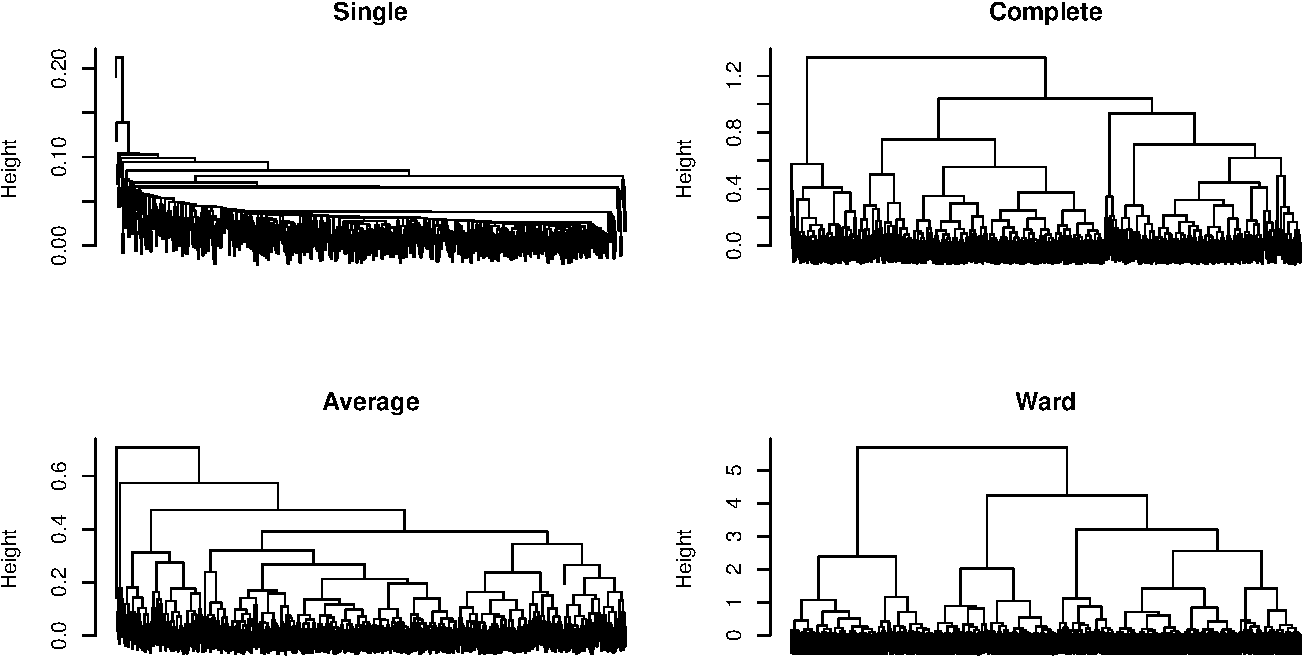
\includegraphics[width=1\linewidth]{pca_report_files/figure-latex/dendrograms-1} 

}

\caption{Four linkage rules on identical shape distances.}\label{fig:dendrograms}
\end{figure}

\begin{Shaded}
\begin{Highlighting}[]
\FunctionTok{par}\NormalTok{(}\AttributeTok{mfrow =} \FunctionTok{c}\NormalTok{(}\DecValTok{1}\NormalTok{, }\DecValTok{1}\NormalTok{))}
\end{Highlighting}
\end{Shaded}

\textbf{Reading:} Leaves are pockets; branches record joins. Height is
the criterion's joining value, not a pocket measurement. Heights are not
directly comparable across criteria. Single shows strong chaining;
average has a dominant branch; complete and Ward are more branched. Ward
has clearer main branches and large final joins. No partition is chosen
from this view alone.

\subsection{Cut at k = 4: cluster sizes and
ARI}\label{cut-at-k-4-cluster-sizes-and-ari}

\texttt{cutree()} assigns groups; \texttt{table()} counts their members.
Four groups are provisional, as required by the assignment.

\begin{Shaded}
\begin{Highlighting}[]
\CommentTok{\# Cut each tree into four groups and compare their sizes.}
\NormalTok{cluster\_single }\OtherTok{\textless{}{-}} \FunctionTok{cutree}\NormalTok{(tree\_single, }\AttributeTok{k =} \DecValTok{4}\NormalTok{)}
\NormalTok{cluster\_complete }\OtherTok{\textless{}{-}} \FunctionTok{cutree}\NormalTok{(tree\_complete, }\AttributeTok{k =} \DecValTok{4}\NormalTok{)}
\NormalTok{cluster\_average }\OtherTok{\textless{}{-}} \FunctionTok{cutree}\NormalTok{(tree\_average, }\AttributeTok{k =} \DecValTok{4}\NormalTok{)}
\NormalTok{cluster\_ward }\OtherTok{\textless{}{-}} \FunctionTok{cutree}\NormalTok{(tree\_ward, }\AttributeTok{k =} \DecValTok{4}\NormalTok{)}
\NormalTok{size\_table }\OtherTok{\textless{}{-}} \FunctionTok{cbind}\NormalTok{(}\AttributeTok{single =} \FunctionTok{table}\NormalTok{(cluster\_single),}
                    \AttributeTok{complete =} \FunctionTok{table}\NormalTok{(cluster\_complete),}
                    \AttributeTok{average =} \FunctionTok{table}\NormalTok{(cluster\_average),}
                    \AttributeTok{ward.D2 =} \FunctionTok{table}\NormalTok{(cluster\_ward))}
\NormalTok{size\_table}
\end{Highlighting}
\end{Shaded}

\begin{verbatim}
##   single complete average ward.D2
## 1    595      289     496     145
## 2      1       80      94     219
## 3      1      214       2     169
## 4      3       17       8      67
\end{verbatim}

\textbf{Table:} Rows are group numbers, columns are methods, entries are
pocket counts. Each column totals 600. Group numbers need not match
across methods. Single gives 595/1/1/3; average 496/94/2/8; complete
289/80/214/17; Ward 145/219/169/67. Ward avoids tiny outlier groups.

\textbf{What is ARI?} The adjusted Rand index asks: do two methods group
the same pockets together? It compares pairs of pockets. A pair agrees
if both methods put it together, or both put it apart. It disagrees if
only one method puts it together. The adjustment accounts for agreement
expected by chance, given the group sizes.

\begin{itemize}
\tightlist
\item
  \textbf{1:} identical grouping, even if the cluster numbers are
  renamed.
\item
  \textbf{Near 0:} agreement is about what chance would produce, not
  zero overlap.
\item
  \textbf{Negative:} less agreement than expected by chance.
\end{itemize}

Higher ARI means more similar memberships. It does not show that groups
are biologically correct or well separated, and it is not a percentage
of matching pockets. We use it here to check how much changing linkage
changes the partition. \texttt{comparison\$corrected.rand} extracts ARI;
the loops compare every pair of methods.

\begin{Shaded}
\begin{Highlighting}[]
\CommentTok{\# Compare every pair of partitions; extract only the ARI.}
\NormalTok{memberships }\OtherTok{\textless{}{-}} \FunctionTok{list}\NormalTok{(cluster\_single, cluster\_complete,}
\NormalTok{                    cluster\_average, cluster\_ward)}
\NormalTok{methods }\OtherTok{\textless{}{-}} \FunctionTok{c}\NormalTok{(}\StringTok{"single"}\NormalTok{, }\StringTok{"complete"}\NormalTok{, }\StringTok{"average"}\NormalTok{, }\StringTok{"ward.D2"}\NormalTok{)}
\NormalTok{ari\_matrix }\OtherTok{\textless{}{-}} \FunctionTok{matrix}\NormalTok{(}\DecValTok{0}\NormalTok{, }\DecValTok{4}\NormalTok{, }\DecValTok{4}\NormalTok{)}
\FunctionTok{rownames}\NormalTok{(ari\_matrix) }\OtherTok{\textless{}{-}}\NormalTok{ methods}
\FunctionTok{colnames}\NormalTok{(ari\_matrix) }\OtherTok{\textless{}{-}}\NormalTok{ methods}
\ControlFlowTok{for}\NormalTok{ (i }\ControlFlowTok{in} \DecValTok{1}\SpecialCharTok{:}\DecValTok{4}\NormalTok{) \{}
  \ControlFlowTok{for}\NormalTok{ (j }\ControlFlowTok{in} \DecValTok{1}\SpecialCharTok{:}\DecValTok{4}\NormalTok{) \{}
\NormalTok{    comparison }\OtherTok{\textless{}{-}}\NormalTok{ fpc}\SpecialCharTok{::}\FunctionTok{cluster.stats}\NormalTok{(dist2, memberships[[i]],}
\NormalTok{                                    memberships[[j]], }\AttributeTok{compareonly =} \ConstantTok{TRUE}\NormalTok{)}
\NormalTok{    ari\_matrix[i, j] }\OtherTok{\textless{}{-}}\NormalTok{ comparison}\SpecialCharTok{$}\NormalTok{corrected.rand}
\NormalTok{  \}}
\NormalTok{\}}
\NormalTok{ari\_matrix}
\end{Highlighting}
\end{Shaded}

\begin{verbatim}
##            single complete average  ward.D2
## single   1.000000 0.005995 0.07788 0.001263
## complete 0.005995 1.000000 0.05789 0.316708
## average  0.077880 0.057887 1.00000 0.146254
## ward.D2  0.001263 0.316708 0.14625 1.000000
\end{verbatim}

\textbf{Table:} Each entry compares its row and column methods. The
diagonal is 1; the two halves repeat comparisons. Complete versus Ward
has ARI 0.317: their grouping agrees only partly. Single versus Ward is
near zero (0.001), so their agreement is near the chance baseline. This
confirms that linkage changes membership.

\subsection{Session 2 summary}\label{session-2-summary}

\textbf{Which rule and why?} Keep Ward: it avoids chaining and produces
more reasonably sized, compact groups. This does not validate k = 4; we
test separation and stability next.

\section{Session 3 --- Choosing k and bootstrap
stability}\label{session-3-choosing-k-and-bootstrap-stability}

\subsection{Rebuild Ward and compare silhouette for k = 2 to
8}\label{rebuild-ward-and-compare-silhouette-for-k-2-to-8}

We rebuild the same unscaled shape tree. Changing only k lets us compare
partitions fairly. A \textbf{silhouette} measures how much better a
pocket fits its own group than the nearest alternative group: near +1 is
well separated, near 0 is a boundary, and negative suggests a better
alternative assignment.

\begin{Shaded}
\begin{Highlighting}[]
\CommentTok{\# Reload and rebuild the same shape clustering.}
\NormalTok{d3 }\OtherTok{\textless{}{-}} \FunctionTok{read.csv}\NormalTok{(}\StringTok{"data\_NS.csv"}\NormalTok{, }\AttributeTok{stringsAsFactors =} \ConstantTok{TRUE}\NormalTok{)}
\NormalTok{x3 }\OtherTok{\textless{}{-}}\NormalTok{ d3[shape\_names]}
\NormalTok{dist3 }\OtherTok{\textless{}{-}} \FunctionTok{dist}\NormalTok{(x3)}
\NormalTok{tree3 }\OtherTok{\textless{}{-}} \FunctionTok{hclust}\NormalTok{(dist3, }\AttributeTok{method =} \StringTok{"ward.D2"}\NormalTok{)}

\CommentTok{\# Average the pocket silhouette scores for each candidate k.}
\NormalTok{ks }\OtherTok{\textless{}{-}} \DecValTok{2}\SpecialCharTok{:}\DecValTok{8}
\NormalTok{silhouette\_mean }\OtherTok{\textless{}{-}} \FunctionTok{numeric}\NormalTok{(}\FunctionTok{length}\NormalTok{(ks))}
\ControlFlowTok{for}\NormalTok{ (i }\ControlFlowTok{in} \DecValTok{1}\SpecialCharTok{:}\FunctionTok{length}\NormalTok{(ks)) \{}
\NormalTok{  groups }\OtherTok{\textless{}{-}} \FunctionTok{cutree}\NormalTok{(tree3, }\AttributeTok{k =}\NormalTok{ ks[i])}
\NormalTok{  pocket\_silhouette }\OtherTok{\textless{}{-}}\NormalTok{ cluster}\SpecialCharTok{::}\FunctionTok{silhouette}\NormalTok{(groups, dist3)}
\NormalTok{  silhouette\_mean[i] }\OtherTok{\textless{}{-}} \FunctionTok{mean}\NormalTok{(pocket\_silhouette[, }\StringTok{"sil\_width"}\NormalTok{])}
\NormalTok{\}}
\FunctionTok{data.frame}\NormalTok{(}\AttributeTok{k =}\NormalTok{ ks, }\AttributeTok{Average\_silhouette =}\NormalTok{ silhouette\_mean)}
\end{Highlighting}
\end{Shaded}

\begin{verbatim}
##   k Average_silhouette
## 1 2             0.3113
## 2 3             0.2879
## 3 4             0.2882
## 4 5             0.2872
## 5 6             0.2995
## 6 7             0.3086
## 7 8             0.2958
\end{verbatim}

\begin{Shaded}
\begin{Highlighting}[]
\NormalTok{best\_k }\OtherTok{\textless{}{-}}\NormalTok{ ks[}\FunctionTok{which.max}\NormalTok{(silhouette\_mean)]}
\end{Highlighting}
\end{Shaded}

\textbf{Columns:} \texttt{k} is the number of groups;
\texttt{Average\_silhouette} is the average score from -1 to +1, not a
percentage.

\begin{Shaded}
\begin{Highlighting}[]
\CommentTok{\# Contrast small score differences with their absolute strength.}
\FunctionTok{par}\NormalTok{(}\AttributeTok{mfrow =} \FunctionTok{c}\NormalTok{(}\DecValTok{1}\NormalTok{, }\DecValTok{2}\NormalTok{), }\AttributeTok{mar =} \FunctionTok{c}\NormalTok{(}\DecValTok{4}\NormalTok{, }\DecValTok{4}\NormalTok{, }\DecValTok{3}\NormalTok{, }\DecValTok{1}\NormalTok{))}
\FunctionTok{plot}\NormalTok{(ks, silhouette\_mean, }\AttributeTok{type =} \StringTok{"b"}\NormalTok{, }\AttributeTok{pch =} \DecValTok{16}\NormalTok{,}
     \AttributeTok{xlab =} \StringTok{"k"}\NormalTok{, }\AttributeTok{ylab =} \StringTok{"Average silhouette"}\NormalTok{, }\AttributeTok{main =} \StringTok{"Default scale"}\NormalTok{)}
\FunctionTok{plot}\NormalTok{(ks, silhouette\_mean, }\AttributeTok{type =} \StringTok{"b"}\NormalTok{, }\AttributeTok{pch =} \DecValTok{16}\NormalTok{, }\AttributeTok{ylim =} \FunctionTok{c}\NormalTok{(}\SpecialCharTok{{-}}\DecValTok{1}\NormalTok{, }\DecValTok{1}\NormalTok{),}
     \AttributeTok{xlab =} \StringTok{"k"}\NormalTok{, }\AttributeTok{ylab =} \StringTok{"Average silhouette"}\NormalTok{, }\AttributeTok{main =} \StringTok{"Full scale [{-}1, 1]"}\NormalTok{)}
\FunctionTok{abline}\NormalTok{(}\AttributeTok{h =} \FloatTok{0.25}\NormalTok{, }\AttributeTok{col =} \StringTok{"\#D95F02"}\NormalTok{, }\AttributeTok{lty =} \DecValTok{2}\NormalTok{)}
\FunctionTok{abline}\NormalTok{(}\AttributeTok{h =} \FloatTok{0.5}\NormalTok{, }\AttributeTok{col =} \StringTok{"\#33A02C"}\NormalTok{, }\AttributeTok{lty =} \DecValTok{2}\NormalTok{)}
\end{Highlighting}
\end{Shaded}

\begin{figure}[H]

{\centering 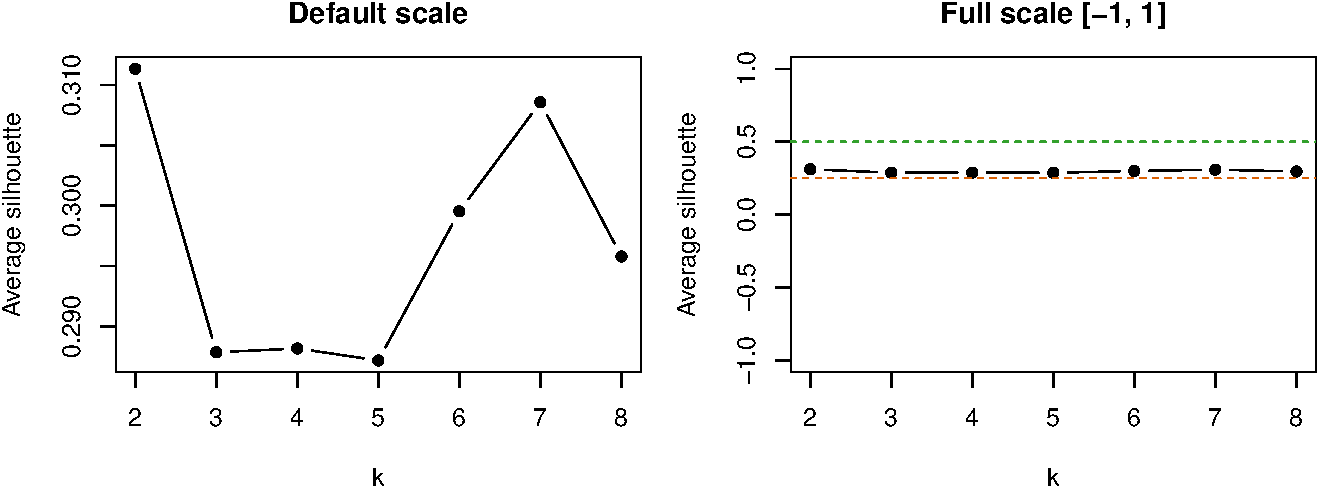
\includegraphics[width=1\linewidth]{pca_report_files/figure-latex/silhouette-scales-1} 

}

\caption{The same scores on the default and full theoretical scales.}\label{fig:silhouette-scales}
\end{figure}

\begin{Shaded}
\begin{Highlighting}[]
\FunctionTok{par}\NormalTok{(}\AttributeTok{mfrow =} \FunctionTok{c}\NormalTok{(}\DecValTok{1}\NormalTok{, }\DecValTok{1}\NormalTok{))}
\end{Highlighting}
\end{Shaded}

\textbf{Optimal k? High score?} k = 2 is best at 0.311, but separation
is weak. The default scale highlights small differences; the full scale
shows all scores are modest, well below 0.5. The reference lines are
guides, not significance tests.

\subsection{Bootstrap stability: k = 4, then 2 and
3}\label{bootstrap-stability-k-4-then-2-and-3}

Bootstrap asks whether groups survive a changed sample. We draw 600
indices with replacement, rebuild Ward, and match each original group to
the new group with maximum \textbf{Jaccard overlap}: shared members
divided by all distinct members. It ranges from 0 (no overlap) to 1
(identical sets).

We compare only sampled identities, counting duplicates once in the
overlap sets. This avoids penalizing absent pockets. All copies still
enter clustering. Each group gets its best match; matching is not forced
to be one-to-one.

\begin{Shaded}
\begin{Highlighting}[]
\CommentTok{\# Run 500 reproducible resamples at each k.}
\NormalTok{B }\OtherTok{\textless{}{-}} \DecValTok{500}
\FunctionTok{set.seed}\NormalTok{(}\DecValTok{22518830}\NormalTok{)}
\NormalTok{stability }\OtherTok{\textless{}{-}} \FunctionTok{list}\NormalTok{()}
\NormalTok{stability\_table }\OtherTok{\textless{}{-}} \FunctionTok{data.frame}\NormalTok{()}
\ControlFlowTok{for}\NormalTok{ (k }\ControlFlowTok{in} \FunctionTok{c}\NormalTok{(}\DecValTok{4}\NormalTok{, }\DecValTok{2}\NormalTok{, }\DecValTok{3}\NormalTok{)) \{}
\NormalTok{  original }\OtherTok{\textless{}{-}} \FunctionTok{cutree}\NormalTok{(tree3, }\AttributeTok{k =}\NormalTok{ k)}
\NormalTok{  scores }\OtherTok{\textless{}{-}} \FunctionTok{matrix}\NormalTok{(}\ConstantTok{NA\_real\_}\NormalTok{, B, k)}
  \ControlFlowTok{for}\NormalTok{ (b }\ControlFlowTok{in} \DecValTok{1}\SpecialCharTok{:}\NormalTok{B) \{}
    \CommentTok{\# Resample and rebuild groups in the same shape space.}
\NormalTok{    ids }\OtherTok{\textless{}{-}} \FunctionTok{sample}\NormalTok{(}\DecValTok{1}\SpecialCharTok{:}\FunctionTok{nrow}\NormalTok{(x3), }\FunctionTok{nrow}\NormalTok{(x3), }\AttributeTok{replace =} \ConstantTok{TRUE}\NormalTok{)}
\NormalTok{    bootstrap\_tree }\OtherTok{\textless{}{-}} \FunctionTok{hclust}\NormalTok{(}\FunctionTok{dist}\NormalTok{(x3[ids, ]), }\AttributeTok{method =} \StringTok{"ward.D2"}\NormalTok{)}
\NormalTok{    bootstrap\_groups }\OtherTok{\textless{}{-}} \FunctionTok{cutree}\NormalTok{(bootstrap\_tree, }\AttributeTok{k =}\NormalTok{ k)}
\NormalTok{    present }\OtherTok{\textless{}{-}} \FunctionTok{unique}\NormalTok{(ids)}
    \ControlFlowTok{for}\NormalTok{ (g }\ControlFlowTok{in} \DecValTok{1}\SpecialCharTok{:}\NormalTok{k) \{}
\NormalTok{      reference }\OtherTok{\textless{}{-}} \FunctionTok{intersect}\NormalTok{(}\FunctionTok{which}\NormalTok{(original }\SpecialCharTok{==}\NormalTok{ g), present)}
      \ControlFlowTok{if}\NormalTok{ (}\FunctionTok{length}\NormalTok{(reference) }\SpecialCharTok{==} \DecValTok{0}\NormalTok{) }\ControlFlowTok{next}
\NormalTok{      matches }\OtherTok{\textless{}{-}} \FunctionTok{numeric}\NormalTok{(k)}
      \ControlFlowTok{for}\NormalTok{ (h }\ControlFlowTok{in} \DecValTok{1}\SpecialCharTok{:}\NormalTok{k) \{}
        \CommentTok{\# Calculate overlap with each candidate group.}
\NormalTok{        candidate }\OtherTok{\textless{}{-}} \FunctionTok{unique}\NormalTok{(ids[bootstrap\_groups }\SpecialCharTok{==}\NormalTok{ h])}
\NormalTok{        shared }\OtherTok{\textless{}{-}} \FunctionTok{length}\NormalTok{(}\FunctionTok{intersect}\NormalTok{(reference, candidate))}
\NormalTok{        total }\OtherTok{\textless{}{-}} \FunctionTok{length}\NormalTok{(}\FunctionTok{union}\NormalTok{(reference, candidate))}
\NormalTok{        matches[h] }\OtherTok{\textless{}{-}}\NormalTok{ shared }\SpecialCharTok{/}\NormalTok{ total}
\NormalTok{      \}}
\NormalTok{      scores[b, g] }\OtherTok{\textless{}{-}} \FunctionTok{max}\NormalTok{(matches)}
\NormalTok{    \}}
\NormalTok{  \}}
  \CommentTok{\# Average each group\textquotesingle{}s best overlap across resamples.}
\NormalTok{  mean\_jaccard }\OtherTok{\textless{}{-}} \FunctionTok{colMeans}\NormalTok{(scores, }\AttributeTok{na.rm =} \ConstantTok{TRUE}\NormalTok{)}
\NormalTok{  stability[[}\FunctionTok{as.character}\NormalTok{(k)]] }\OtherTok{\textless{}{-}}\NormalTok{ mean\_jaccard}
\NormalTok{  stability\_table }\OtherTok{\textless{}{-}} \FunctionTok{rbind}\NormalTok{(stability\_table,}
    \FunctionTok{data.frame}\NormalTok{(}\AttributeTok{k =}\NormalTok{ k, }\AttributeTok{Cluster =} \DecValTok{1}\SpecialCharTok{:}\NormalTok{k, }\AttributeTok{Mean\_Jaccard =}\NormalTok{ mean\_jaccard))}
\NormalTok{\}}
\NormalTok{stability\_table}
\end{Highlighting}
\end{Shaded}

\begin{verbatim}
##   k Cluster Mean_Jaccard
## 1 4       1       0.5104
## 2 4       2       0.3917
## 3 4       3       0.5633
## 4 4       4       0.4572
## 5 2       1       0.7135
## 6 2       2       0.5970
## 7 3       1       0.4902
## 8 3       2       0.4760
## 9 3       3       0.5979
\end{verbatim}

\begin{Shaded}
\begin{Highlighting}[]
\FunctionTok{aggregate}\NormalTok{(Mean\_Jaccard }\SpecialCharTok{\textasciitilde{}}\NormalTok{ k, }\AttributeTok{data =}\NormalTok{ stability\_table, }\AttributeTok{FUN =}\NormalTok{ mean)}
\end{Highlighting}
\end{Shaded}

\begin{verbatim}
##   k Mean_Jaccard
## 1 2       0.6553
## 2 3       0.5214
## 3 4       0.4806
\end{verbatim}

\textbf{Columns:} \texttt{k} identifies the partition; \texttt{Cluster}
is its original group; \texttt{Mean\_Jaccard} is its mean best overlap
over 500 resamples. The final table averages across groups, weighting
each group equally. Missing comparisons are omitted if a group has no
sampled member.

\textbf{Answer:} k = 4 scores range from 0.392 to 0.563, showing
instability. k = 2 gives 0.714 and 0.597, better but limited. k = 3
gives 0.49, 0.476, 0.598. None reaches the usual 0.75 mean-Jaccard
stability guideline. We retain four groups in session 4 only for the
requested comparison.

\subsection{Session 3 summary}\label{session-3-summary}

\textbf{Same question?} No.~Silhouette measures observed separation;
bootstrap measures reproducibility under resampling. Both favor k = 2
here, but neither strongly supports clearly separated natural groups.

\section{Session 4 --- Clustering, PCA, and
heatmap}\label{session-4-clustering-pca-and-heatmap}

\subsection{Repeat shape clustering and add scaled shape-plus-size
clustering}\label{repeat-shape-clustering-and-add-scaled-shape-plus-size-clustering}

We compare the same pockets at k = 4. The first tree exactly repeats the
previous unscaled ratios; the second adds size and therefore requires
scaling.

\begin{Shaded}
\begin{Highlighting}[]
\CommentTok{\# Reload, recompute Rg, and prepare the two measurement spaces.}
\NormalTok{d4 }\OtherTok{\textless{}{-}} \FunctionTok{read.csv}\NormalTok{(}\StringTok{"data\_NS.csv"}\NormalTok{, }\AttributeTok{stringsAsFactors =} \ConstantTok{TRUE}\NormalTok{)}
\NormalTok{d4}\SpecialCharTok{$}\NormalTok{Rg }\OtherTok{\textless{}{-}} \FunctionTok{sqrt}\NormalTok{(d4}\SpecialCharTok{$}\NormalTok{Eigval}\FloatTok{.1} \SpecialCharTok{+}\NormalTok{ d4}\SpecialCharTok{$}\NormalTok{Eigval}\FloatTok{.2} \SpecialCharTok{+}\NormalTok{ d4}\SpecialCharTok{$}\NormalTok{Eigval}\FloatTok{.3}\NormalTok{)}
\NormalTok{x4 }\OtherTok{\textless{}{-}}\NormalTok{ d4[shape\_names]}
\NormalTok{z4 }\OtherTok{\textless{}{-}} \FunctionTok{scale}\NormalTok{(d4[five\_names])}
\NormalTok{dist\_shape }\OtherTok{\textless{}{-}} \FunctionTok{dist}\NormalTok{(x4)}
\NormalTok{dist\_five }\OtherTok{\textless{}{-}} \FunctionTok{dist}\NormalTok{(z4)}

\CommentTok{\# Build both Ward partitions and check the repeated one is unchanged.}
\NormalTok{tree\_shape }\OtherTok{\textless{}{-}} \FunctionTok{hclust}\NormalTok{(dist\_shape, }\AttributeTok{method =} \StringTok{"ward.D2"}\NormalTok{)}
\NormalTok{tree\_five }\OtherTok{\textless{}{-}} \FunctionTok{hclust}\NormalTok{(dist\_five, }\AttributeTok{method =} \StringTok{"ward.D2"}\NormalTok{)}
\NormalTok{cluster\_shape }\OtherTok{\textless{}{-}} \FunctionTok{cutree}\NormalTok{(tree\_shape, }\AttributeTok{k =} \DecValTok{4}\NormalTok{)}
\NormalTok{cluster\_five }\OtherTok{\textless{}{-}} \FunctionTok{cutree}\NormalTok{(tree\_five, }\AttributeTok{k =} \DecValTok{4}\NormalTok{)}
\FunctionTok{identical}\NormalTok{(cluster\_shape, }\FunctionTok{cutree}\NormalTok{(tree3, }\AttributeTok{k =} \DecValTok{4}\NormalTok{))}
\end{Highlighting}
\end{Shaded}

\begin{verbatim}
## [1] TRUE
\end{verbatim}

\begin{Shaded}
\begin{Highlighting}[]
\FunctionTok{cor}\NormalTok{(d4}\SpecialCharTok{$}\NormalTok{Num\_Atoms, d4}\SpecialCharTok{$}\NormalTok{Rg)}
\end{Highlighting}
\end{Shaded}

\begin{verbatim}
## [1] 0.8297
\end{verbatim}

\textbf{Size weighting:} Atom count and \texttt{Rg} correlate at about
0.83, partly repeating size information. Including both gives size more
weight than using one descriptor. Scaling equalizes variances, not
independent biological features; the shape ratios also contain
redundancy.

\subsection{Rebuild PCA1 and PCA2; show Origin and both
clusterings}\label{rebuild-pca1-and-pca2-show-origin-and-both-clusterings}

PCA summarizes the measurement spaces; cluster colors describe their
groups. Origin remains supplementary in both PCAs.

\begin{Shaded}
\begin{Highlighting}[]
\CommentTok{\# Repeat the PCAs from session 1 without using group labels to define axes.}
\NormalTok{pca1\_4 }\OtherTok{\textless{}{-}} \FunctionTok{PCA}\NormalTok{(d4[}\FunctionTok{c}\NormalTok{(shape\_names, }\StringTok{"Origin"}\NormalTok{)], }\AttributeTok{scale.unit =} \ConstantTok{FALSE}\NormalTok{,}
              \AttributeTok{quali.sup =} \DecValTok{4}\NormalTok{, }\AttributeTok{graph =} \ConstantTok{FALSE}\NormalTok{)}
\NormalTok{pca2\_4 }\OtherTok{\textless{}{-}} \FunctionTok{PCA}\NormalTok{(d4[}\FunctionTok{c}\NormalTok{(five\_names, }\StringTok{"Origin"}\NormalTok{)], }\AttributeTok{scale.unit =} \ConstantTok{TRUE}\NormalTok{,}
              \AttributeTok{quali.sup =} \DecValTok{6}\NormalTok{, }\AttributeTok{graph =} \ConstantTok{FALSE}\NormalTok{)}
\end{Highlighting}
\end{Shaded}

\begin{Shaded}
\begin{Highlighting}[]
\CommentTok{\# Show known Origins on the shape{-}plus{-}size scores.}
\FunctionTok{plot}\NormalTok{(pca2\_4, }\AttributeTok{choix =} \StringTok{"ind"}\NormalTok{, }\AttributeTok{habillage =} \DecValTok{6}\NormalTok{, }\AttributeTok{label =} \StringTok{"none"}\NormalTok{,}
     \AttributeTok{title =} \StringTok{"Shape + size PCA: Origin"}\NormalTok{)}
\end{Highlighting}
\end{Shaded}

\begin{figure}[H]

{\centering 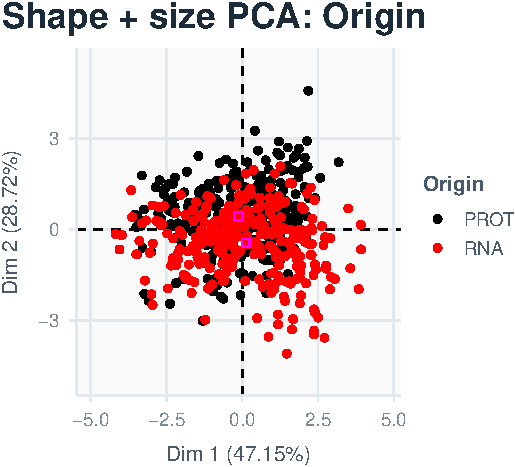
\includegraphics[width=0.72\linewidth]{pca_report_files/figure-latex/origin-pca2-1} 

}

\caption{Supplementary Origin on the scaled shape-plus-size PCA.}\label{fig:origin-pca2}
\end{figure}

\textbf{Origin:} RNA and proteins still overlap, but show a shift along
size-related variation. RNA pockets have more atoms and larger mean
\texttt{Rg}.

We now keep the same pure-shape coordinates and change only the colors.
This tests whether the size-influenced groups are visible using shape
alone.

\begin{Shaded}
\begin{Highlighting}[]
\CommentTok{\# Use the same shape{-}only scores in both panels.}
\NormalTok{pc1 }\OtherTok{\textless{}{-}}\NormalTok{ pca1\_4}\SpecialCharTok{$}\NormalTok{ind}\SpecialCharTok{$}\NormalTok{coord[, }\DecValTok{1}\NormalTok{]}
\NormalTok{pc2 }\OtherTok{\textless{}{-}}\NormalTok{ pca1\_4}\SpecialCharTok{$}\NormalTok{ind}\SpecialCharTok{$}\NormalTok{coord[, }\DecValTok{2}\NormalTok{]}
\FunctionTok{par}\NormalTok{(}\AttributeTok{mfrow =} \FunctionTok{c}\NormalTok{(}\DecValTok{1}\NormalTok{, }\DecValTok{2}\NormalTok{), }\AttributeTok{mar =} \FunctionTok{c}\NormalTok{(}\DecValTok{4}\NormalTok{, }\DecValTok{4}\NormalTok{, }\DecValTok{3}\NormalTok{, }\DecValTok{1}\NormalTok{))}
\FunctionTok{plot}\NormalTok{(pc1, pc2, }\AttributeTok{col =}\NormalTok{ cluster\_colors[cluster\_five], }\AttributeTok{pch =} \DecValTok{16}\NormalTok{, }\AttributeTok{cex =} \FloatTok{0.5}\NormalTok{,}
     \AttributeTok{xlab =} \StringTok{"PC1 (59.74\%)"}\NormalTok{, }\AttributeTok{ylab =} \StringTok{"PC2 (39.52\%)"}\NormalTok{,}
     \AttributeTok{main =} \StringTok{"Five{-}variable groups"}\NormalTok{)}
\FunctionTok{legend}\NormalTok{(}\StringTok{"topright"}\NormalTok{, }\AttributeTok{legend =} \DecValTok{1}\SpecialCharTok{:}\DecValTok{4}\NormalTok{, }\AttributeTok{col =}\NormalTok{ cluster\_colors, }\AttributeTok{pch =} \DecValTok{16}\NormalTok{, }\AttributeTok{bty =} \StringTok{"n"}\NormalTok{)}
\FunctionTok{plot}\NormalTok{(pc1, pc2, }\AttributeTok{col =}\NormalTok{ cluster\_colors[cluster\_shape], }\AttributeTok{pch =} \DecValTok{16}\NormalTok{, }\AttributeTok{cex =} \FloatTok{0.5}\NormalTok{,}
     \AttributeTok{xlab =} \StringTok{"PC1 (59.74\%)"}\NormalTok{, }\AttributeTok{ylab =} \StringTok{"PC2 (39.52\%)"}\NormalTok{,}
     \AttributeTok{main =} \StringTok{"Shape{-}only groups"}\NormalTok{)}
\FunctionTok{legend}\NormalTok{(}\StringTok{"topright"}\NormalTok{, }\AttributeTok{legend =} \DecValTok{1}\SpecialCharTok{:}\DecValTok{4}\NormalTok{, }\AttributeTok{col =}\NormalTok{ cluster\_colors, }\AttributeTok{pch =} \DecValTok{16}\NormalTok{, }\AttributeTok{bty =} \StringTok{"n"}\NormalTok{)}
\end{Highlighting}
\end{Shaded}

\begin{figure}[H]

{\centering 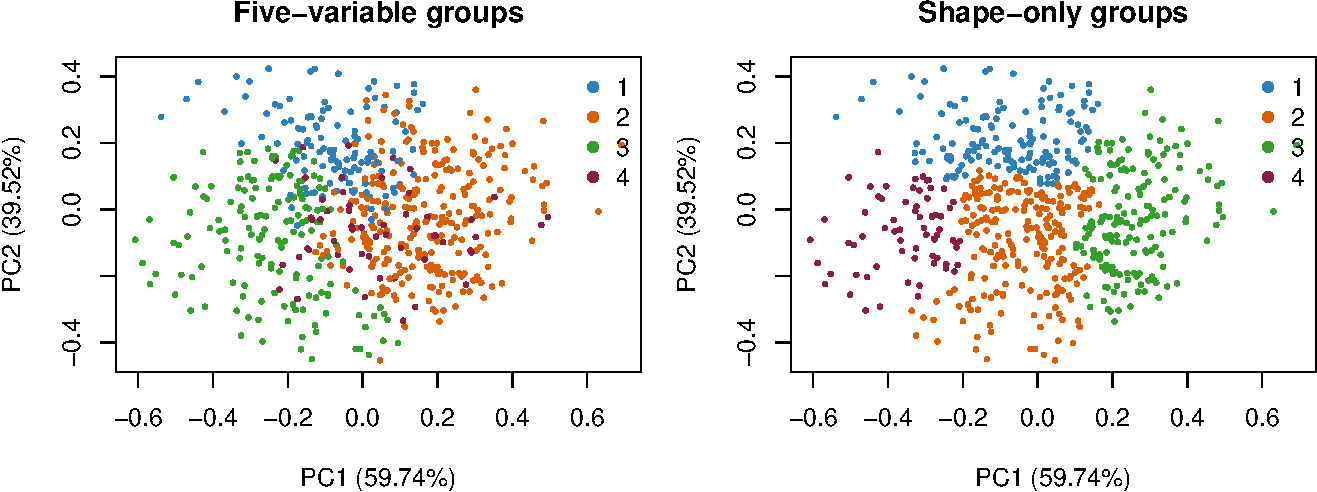
\includegraphics[width=1\linewidth]{pca_report_files/figure-latex/clusters-on-shape-1} 

}

\caption{Identical shape coordinates colored by the five-variable and shape-only groups.}\label{fig:clusters-on-shape}
\end{figure}

\begin{Shaded}
\begin{Highlighting}[]
\FunctionTok{par}\NormalTok{(}\AttributeTok{mfrow =} \FunctionTok{c}\NormalTok{(}\DecValTok{1}\NormalTok{, }\DecValTok{1}\NormalTok{))}
\end{Highlighting}
\end{Shaded}

\textbf{Visible size trace?} Partly: five-variable groups show some
shape differences but overlap more. Their very large-pocket group does
not form a distinct shape region. Shape-only colors form clearer regions
because those groups were built from shape. Shape cannot fully recover
the organization added by size.

\subsection{Heatmap and numerical
comparison}\label{heatmap-and-numerical-comparison}

Rows are pockets; columns are the five measurements. Values are
standardized: 0 is the mean, +1 is one SD above, and -1 one SD below.
Blue means lower, white near average, and red higher. The five-variable
Ward tree orders rows; side bars identify Origin and both group
assignments.

\begin{Shaded}
\begin{Highlighting}[]
\CommentTok{\# Match the measurements and category annotations by pocket row.}
\NormalTok{annotation }\OtherTok{\textless{}{-}} \FunctionTok{data.frame}\NormalTok{(}\AttributeTok{Origin =}\NormalTok{ d4}\SpecialCharTok{$}\NormalTok{Origin,}
                         \AttributeTok{Cluster\_five =} \FunctionTok{factor}\NormalTok{(cluster\_five),}
                         \AttributeTok{Cluster\_shape =} \FunctionTok{factor}\NormalTok{(cluster\_shape))}
\FunctionTok{rownames}\NormalTok{(z4) }\OtherTok{\textless{}{-}} \FunctionTok{paste0}\NormalTok{(}\StringTok{"Pocket\_"}\NormalTok{, }\DecValTok{1}\SpecialCharTok{:}\FunctionTok{nrow}\NormalTok{(d4))}
\FunctionTok{rownames}\NormalTok{(annotation) }\OtherTok{\textless{}{-}} \FunctionTok{rownames}\NormalTok{(z4)}
\NormalTok{annotation\_colors }\OtherTok{\textless{}{-}} \FunctionTok{list}\NormalTok{(}
  \AttributeTok{Origin =}\NormalTok{ origin\_colors,}
  \AttributeTok{Cluster\_five =} \FunctionTok{setNames}\NormalTok{(cluster\_colors, }\DecValTok{1}\SpecialCharTok{:}\DecValTok{4}\NormalTok{),}
  \AttributeTok{Cluster\_shape =} \FunctionTok{setNames}\NormalTok{(cluster\_colors, }\DecValTok{1}\SpecialCharTok{:}\DecValTok{4}\NormalTok{))}

\CommentTok{\# Reuse the five{-}variable tree and retain the stated column order.}
\FunctionTok{pheatmap}\NormalTok{(z4, }\AttributeTok{cluster\_rows =}\NormalTok{ tree\_five, }\AttributeTok{cluster\_cols =} \ConstantTok{FALSE}\NormalTok{,}
         \AttributeTok{annotation\_row =}\NormalTok{ annotation, }\AttributeTok{annotation\_colors =}\NormalTok{ annotation\_colors,}
         \AttributeTok{show\_rownames =} \ConstantTok{FALSE}\NormalTok{, }\AttributeTok{border\_color =} \ConstantTok{NA}\NormalTok{,}
         \AttributeTok{color =} \FunctionTok{hcl.colors}\NormalTok{(}\DecValTok{100}\NormalTok{, }\StringTok{"Blue{-}Red 3"}\NormalTok{), }\AttributeTok{fontsize =} \DecValTok{9}\NormalTok{)}
\end{Highlighting}
\end{Shaded}

\begin{figure}[H]

{\centering 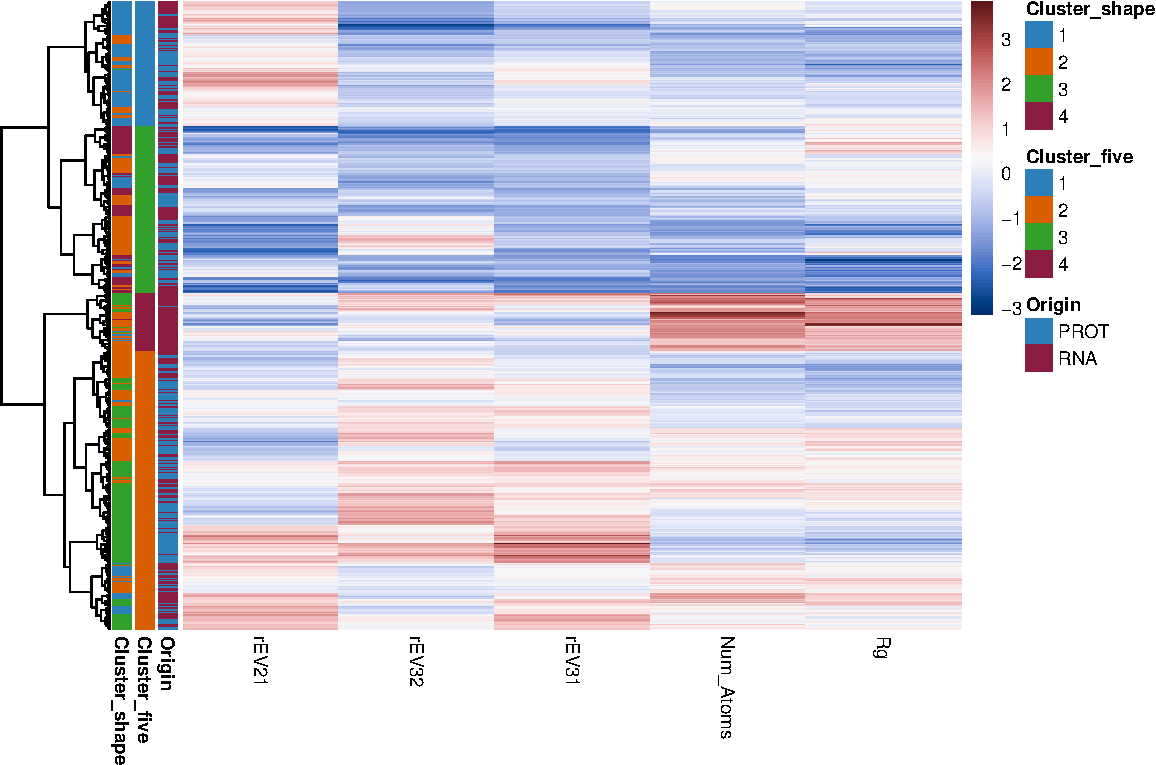
\includegraphics[width=1\linewidth]{pca_report_files/figure-latex/heatmap-1} 

}

\caption{Standardized measurements ordered by the five-variable Ward tree.}\label{fig:heatmap}
\end{figure}

\textbf{Do blocks line up?} Five-variable groups form contiguous blocks
because their own tree orders the rows. Shape-only groups are more
mixed; Origin is also mixed. Matching colors across the two group bars
do not automatically mean matching groups.

\begin{Shaded}
\begin{Highlighting}[]
\CommentTok{\# Count shared members: shape groups in rows, five{-}variable groups in columns.}
\NormalTok{cross\_table }\OtherTok{\textless{}{-}} \FunctionTok{table}\NormalTok{(}\AttributeTok{Shape =}\NormalTok{ cluster\_shape, }\AttributeTok{Five =}\NormalTok{ cluster\_five)}
\NormalTok{cross\_table}
\end{Highlighting}
\end{Shaded}

\begin{verbatim}
##      Five
## Shape   1   2   3   4
##     1  92  27  21   5
##     2  26  88  73  32
##     3   1 151   0  17
##     4   0   0  66   1
\end{verbatim}

\begin{Shaded}
\begin{Highlighting}[]
\CommentTok{\# Convert shared counts into Jaccard overlaps for every group pair.}
\NormalTok{jaccard\_matrix }\OtherTok{\textless{}{-}} \FunctionTok{matrix}\NormalTok{(}\DecValTok{0}\NormalTok{, }\DecValTok{4}\NormalTok{, }\DecValTok{4}\NormalTok{)}
\FunctionTok{rownames}\NormalTok{(jaccard\_matrix) }\OtherTok{\textless{}{-}} \FunctionTok{paste}\NormalTok{(}\StringTok{"Shape"}\NormalTok{, }\DecValTok{1}\SpecialCharTok{:}\DecValTok{4}\NormalTok{)}
\FunctionTok{colnames}\NormalTok{(jaccard\_matrix) }\OtherTok{\textless{}{-}} \FunctionTok{paste}\NormalTok{(}\StringTok{"Five"}\NormalTok{, }\DecValTok{1}\SpecialCharTok{:}\DecValTok{4}\NormalTok{)}
\ControlFlowTok{for}\NormalTok{ (i }\ControlFlowTok{in} \DecValTok{1}\SpecialCharTok{:}\DecValTok{4}\NormalTok{) \{}
  \ControlFlowTok{for}\NormalTok{ (j }\ControlFlowTok{in} \DecValTok{1}\SpecialCharTok{:}\DecValTok{4}\NormalTok{) \{}
\NormalTok{    shared }\OtherTok{\textless{}{-}}\NormalTok{ cross\_table[i, j]}
\NormalTok{    total }\OtherTok{\textless{}{-}} \FunctionTok{sum}\NormalTok{(cross\_table[i, ]) }\SpecialCharTok{+} \FunctionTok{sum}\NormalTok{(cross\_table[, j]) }\SpecialCharTok{{-}}\NormalTok{ shared}
\NormalTok{    jaccard\_matrix[i, j] }\OtherTok{\textless{}{-}}\NormalTok{ shared }\SpecialCharTok{/}\NormalTok{ total}
\NormalTok{  \}}
\NormalTok{\}}
\NormalTok{jaccard\_matrix}
\end{Highlighting}
\end{Shaded}

\begin{verbatim}
##           Five 1  Five 2  Five 3   Five 4
## Shape 1 0.534884 0.07031 0.07394 0.025641
## Shape 2 0.083333 0.22166 0.23856 0.132231
## Shape 3 0.003484 0.53169 0.00000 0.082126
## Shape 4 0.000000 0.00000 0.40994 0.008264
\end{verbatim}

\begin{Shaded}
\begin{Highlighting}[]
\CommentTok{\# Find the best match for each shape group.}
\NormalTok{best\_matches }\OtherTok{\textless{}{-}} \FunctionTok{data.frame}\NormalTok{(}\AttributeTok{Shape\_cluster =} \DecValTok{1}\SpecialCharTok{:}\DecValTok{4}\NormalTok{,}
                          \AttributeTok{Best\_five\_cluster =} \FunctionTok{integer}\NormalTok{(}\DecValTok{4}\NormalTok{),}
                          \AttributeTok{Best\_Jaccard =} \FunctionTok{numeric}\NormalTok{(}\DecValTok{4}\NormalTok{))}
\ControlFlowTok{for}\NormalTok{ (i }\ControlFlowTok{in} \DecValTok{1}\SpecialCharTok{:}\DecValTok{4}\NormalTok{) \{}
\NormalTok{  best\_matches}\SpecialCharTok{$}\NormalTok{Best\_five\_cluster[i] }\OtherTok{\textless{}{-}} \FunctionTok{which.max}\NormalTok{(jaccard\_matrix[i, ])}
\NormalTok{  best\_matches}\SpecialCharTok{$}\NormalTok{Best\_Jaccard[i] }\OtherTok{\textless{}{-}} \FunctionTok{max}\NormalTok{(jaccard\_matrix[i, ])}
\NormalTok{\}}
\NormalTok{best\_matches}
\end{Highlighting}
\end{Shaded}

\begin{verbatim}
##   Shape_cluster Best_five_cluster Best_Jaccard
## 1             1                 1       0.5349
## 2             2                 3       0.2386
## 3             3                 2       0.5317
## 4             4                 3       0.4099
\end{verbatim}

\begin{Shaded}
\begin{Highlighting}[]
\CommentTok{\# Compare the complete partitions using ARI.}
\NormalTok{comparison }\OtherTok{\textless{}{-}}\NormalTok{ fpc}\SpecialCharTok{::}\FunctionTok{cluster.stats}\NormalTok{(dist\_shape, cluster\_shape, cluster\_five,}
                                 \AttributeTok{compareonly =} \ConstantTok{TRUE}\NormalTok{)}
\NormalTok{agreement }\OtherTok{\textless{}{-}}\NormalTok{ comparison}\SpecialCharTok{$}\NormalTok{corrected.rand}
\NormalTok{agreement}
\end{Highlighting}
\end{Shaded}

\begin{verbatim}
## [1] 0.2576
\end{verbatim}

\textbf{Tables:} The contingency entries count shared pockets. Jaccard
entries give shared membership divided by combined distinct membership,
between 0 and 1. \texttt{Shape\_cluster} identifies the old group,
\texttt{Best\_five\_cluster} its highest-overlap new group, and
\texttt{Best\_Jaccard} that overlap. Numbers are arbitrary, so the
contingency diagonal has no special meaning.

\textbf{Numerical answer:} Best overlaps are 0.535, 0.239, 0.532, 0.41;
ARI is 0.258. Agreement is partial: adding size changes membership, not
just group names.

\subsection{Final summary connecting the
sessions}\label{final-summary-connecting-the-sessions}

Session 1 separated shape from size and demonstrated why scaling
matters. Session 2 showed that linkage changes memberships, with Ward
avoiding strong chaining. Session 3 found weak separation and limited
reproducibility of four shape groups. Session 4 showed that standardized
size adds a different grouping signal. Together, the results support
overlapping shape variation plus size variation, rather than four firmly
established natural shape groups or two completely separate Origins.

\section{Going further --- Personal
reflection}\label{going-further-personal-reflection}

\subsection{Archetype rule and comparison with both
clusterings}\label{archetype-rule-and-comparison-with-both-clusterings}

\textbf{Limitation:} The complete CSV and detailed QMD named in
\texttt{document.pdf} are absent. If the CSV is unavailable, we
reconstruct the article's rule; these are not independently supplied
labels. Archetypes are median-threshold categories, not Ward results:
high/high ratios give sphere-like, high/low disk-like, low/high
rod-like, and low/low strongly anisotropic shapes.

\begin{Shaded}
\begin{Highlighting}[]
\CommentTok{\# Estimate pooled thresholds and assign all four ratio combinations.}
\NormalTok{median21 }\OtherTok{\textless{}{-}} \FunctionTok{median}\NormalTok{(d4}\SpecialCharTok{$}\NormalTok{rEV21)}
\NormalTok{median32 }\OtherTok{\textless{}{-}} \FunctionTok{median}\NormalTok{(d4}\SpecialCharTok{$}\NormalTok{rEV32)}
\FunctionTok{data.frame}\NormalTok{(}\AttributeTok{Variable =} \FunctionTok{c}\NormalTok{(}\StringTok{"rEV21"}\NormalTok{, }\StringTok{"rEV32"}\NormalTok{),}
           \AttributeTok{Median\_threshold =} \FunctionTok{c}\NormalTok{(median21, median32))}
\end{Highlighting}
\end{Shaded}

\begin{verbatim}
##   Variable Median_threshold
## 1    rEV21           0.5923
## 2    rEV32           0.5751
\end{verbatim}

\begin{Shaded}
\begin{Highlighting}[]
\NormalTok{high21 }\OtherTok{\textless{}{-}}\NormalTok{ d4}\SpecialCharTok{$}\NormalTok{rEV21 }\SpecialCharTok{\textgreater{}=}\NormalTok{ median21}
\NormalTok{high32 }\OtherTok{\textless{}{-}}\NormalTok{ d4}\SpecialCharTok{$}\NormalTok{rEV32 }\SpecialCharTok{\textgreater{}=}\NormalTok{ median32}
\NormalTok{rule\_archetype }\OtherTok{\textless{}{-}} \FunctionTok{rep}\NormalTok{(}\StringTok{"Strongly anisotropic"}\NormalTok{, }\FunctionTok{nrow}\NormalTok{(d4))}
\NormalTok{rule\_archetype[high21 }\SpecialCharTok{\&}\NormalTok{ high32] }\OtherTok{\textless{}{-}} \StringTok{"Sphere{-}like"}
\NormalTok{rule\_archetype[high21 }\SpecialCharTok{\&} \SpecialCharTok{!}\NormalTok{high32] }\OtherTok{\textless{}{-}} \StringTok{"Disk{-}like"}
\NormalTok{rule\_archetype[}\SpecialCharTok{!}\NormalTok{high21 }\SpecialCharTok{\&}\NormalTok{ high32] }\OtherTok{\textless{}{-}} \StringTok{"Rod{-}like"}

\CommentTok{\# Load supplied labels if available, matching pocket identities first.}
\NormalTok{archetype }\OtherTok{\textless{}{-}}\NormalTok{ rule\_archetype}
\NormalTok{label\_source }\OtherTok{\textless{}{-}} \StringTok{"Reconstructed median{-}rule labels"}
\NormalTok{complete\_path }\OtherTok{\textless{}{-}} \StringTok{"../data/2026{-}09{-}09\_data\_PROT\_RNA\_TP\_seance4\_complet.csv"}
\ControlFlowTok{if}\NormalTok{ (}\FunctionTok{file.exists}\NormalTok{(complete\_path)) \{}
\NormalTok{  complete }\OtherTok{\textless{}{-}} \FunctionTok{read.csv}\NormalTok{(complete\_path)}
\NormalTok{  key }\OtherTok{\textless{}{-}} \FunctionTok{paste}\NormalTok{(d4}\SpecialCharTok{$}\NormalTok{PDB\_ID, d4}\SpecialCharTok{$}\NormalTok{Pocket)}
\NormalTok{  complete\_key }\OtherTok{\textless{}{-}} \FunctionTok{paste}\NormalTok{(complete}\SpecialCharTok{$}\NormalTok{PDB\_ID, complete}\SpecialCharTok{$}\NormalTok{Pocket)}
\NormalTok{  index }\OtherTok{\textless{}{-}} \FunctionTok{match}\NormalTok{(key, complete\_key)}
  \FunctionTok{stopifnot}\NormalTok{(}\StringTok{"Archetype"} \SpecialCharTok{\%in\%} \FunctionTok{names}\NormalTok{(complete), }\SpecialCharTok{!}\FunctionTok{anyNA}\NormalTok{(index),}
            \SpecialCharTok{!}\FunctionTok{anyDuplicated}\NormalTok{(complete\_key), }\SpecialCharTok{!}\FunctionTok{anyNA}\NormalTok{(complete}\SpecialCharTok{$}\NormalTok{Archetype[index]))}
\NormalTok{  archetype }\OtherTok{\textless{}{-}}\NormalTok{ complete}\SpecialCharTok{$}\NormalTok{Archetype[index]}
\NormalTok{  label\_source }\OtherTok{\textless{}{-}} \StringTok{"Archetype labels loaded from the complete file"}
\NormalTok{\}}
\NormalTok{label\_source}
\end{Highlighting}
\end{Shaded}

\begin{verbatim}
## [1] "Reconstructed median-rule labels"
\end{verbatim}

\texttt{Variable} names each ratio; \texttt{Median\_threshold} gives its
dividing value. High means at least the median. Identity matching avoids
comparing unrelated rows if the complete file has a different order.

\begin{Shaded}
\begin{Highlighting}[]
\CommentTok{\# Compare each clustering with the rule; integer labels preserve membership.}
\NormalTok{archetype\_labels }\OtherTok{\textless{}{-}} \FunctionTok{as.integer}\NormalTok{(}\FunctionTok{factor}\NormalTok{(archetype))}
\NormalTok{shape\_comparison }\OtherTok{\textless{}{-}}\NormalTok{ fpc}\SpecialCharTok{::}\FunctionTok{cluster.stats}\NormalTok{(dist\_shape, cluster\_shape,}
\NormalTok{                                      archetype\_labels, }\AttributeTok{compareonly =} \ConstantTok{TRUE}\NormalTok{)}
\NormalTok{five\_comparison }\OtherTok{\textless{}{-}}\NormalTok{ fpc}\SpecialCharTok{::}\FunctionTok{cluster.stats}\NormalTok{(dist\_shape, cluster\_five,}
\NormalTok{                                     archetype\_labels, }\AttributeTok{compareonly =} \ConstantTok{TRUE}\NormalTok{)}
\NormalTok{shape\_archetype\_ari }\OtherTok{\textless{}{-}}\NormalTok{ shape\_comparison}\SpecialCharTok{$}\NormalTok{corrected.rand}
\NormalTok{five\_archetype\_ari }\OtherTok{\textless{}{-}}\NormalTok{ five\_comparison}\SpecialCharTok{$}\NormalTok{corrected.rand}
\FunctionTok{data.frame}\NormalTok{(}\AttributeTok{Clustering =} \FunctionTok{c}\NormalTok{(}\StringTok{"Three ratios"}\NormalTok{, }\StringTok{"Five variables"}\NormalTok{),}
           \AttributeTok{ARI\_with\_Archetype =} \FunctionTok{c}\NormalTok{(shape\_archetype\_ari, five\_archetype\_ari))}
\end{Highlighting}
\end{Shaded}

\begin{verbatim}
##       Clustering ARI_with_Archetype
## 1   Three ratios             0.4002
## 2 Five variables             0.2898
\end{verbatim}

\texttt{Clustering} identifies the analysis;
\texttt{ARI\_with\_Archetype} measures its agreement with the
categories. Shape-only ARI is 0.4 versus 0.29 with size. Neither
reproduces the rule exactly; shape-only agrees more because the rule
excludes size.

\subsection{Frequencies and shape-versus-size effect
sizes}\label{frequencies-and-shape-versus-size-effect-sizes}

\begin{Shaded}
\begin{Highlighting}[]
\CommentTok{\# Compare category counts and percentages within each Origin.}
\NormalTok{frequency }\OtherTok{\textless{}{-}} \FunctionTok{table}\NormalTok{(}\AttributeTok{Archetype =}\NormalTok{ archetype, }\AttributeTok{Origin =}\NormalTok{ d4}\SpecialCharTok{$}\NormalTok{Origin)}
\NormalTok{frequency}
\end{Highlighting}
\end{Shaded}

\begin{verbatim}
##                       Origin
## Archetype              PROT RNA
##   Disk-like              74  91
##   Rod-like               80  85
##   Sphere-like            86  49
##   Strongly anisotropic   60  75
\end{verbatim}

\begin{Shaded}
\begin{Highlighting}[]
\DecValTok{100} \SpecialCharTok{*} \FunctionTok{prop.table}\NormalTok{(frequency, }\AttributeTok{margin =} \DecValTok{2}\NormalTok{)}
\end{Highlighting}
\end{Shaded}

\begin{verbatim}
##                       Origin
## Archetype               PROT   RNA
##   Disk-like            24.67 30.33
##   Rod-like             26.67 28.33
##   Sphere-like          28.67 16.33
##   Strongly anisotropic 20.00 25.00
\end{verbatim}

\begin{Shaded}
\begin{Highlighting}[]
\CommentTok{\# Express each RNA{-}minus{-}protein mean difference in pooled SD units.}
\NormalTok{effect\_table }\OtherTok{\textless{}{-}} \FunctionTok{data.frame}\NormalTok{(}\AttributeTok{Variable =}\NormalTok{ five\_names, }\AttributeTok{RNA\_mean =} \FunctionTok{numeric}\NormalTok{(}\DecValTok{5}\NormalTok{),}
                          \AttributeTok{PROT\_mean =} \FunctionTok{numeric}\NormalTok{(}\DecValTok{5}\NormalTok{), }\AttributeTok{Cohen\_d =} \FunctionTok{numeric}\NormalTok{(}\DecValTok{5}\NormalTok{))}
\ControlFlowTok{for}\NormalTok{ (i }\ControlFlowTok{in} \DecValTok{1}\SpecialCharTok{:}\DecValTok{5}\NormalTok{) \{}
\NormalTok{  rna\_values }\OtherTok{\textless{}{-}}\NormalTok{ d4[d4}\SpecialCharTok{$}\NormalTok{Origin }\SpecialCharTok{==} \StringTok{"RNA"}\NormalTok{, five\_names[i]]}
\NormalTok{  protein\_values }\OtherTok{\textless{}{-}}\NormalTok{ d4[d4}\SpecialCharTok{$}\NormalTok{Origin }\SpecialCharTok{==} \StringTok{"PROT"}\NormalTok{, five\_names[i]]}
\NormalTok{  pooled\_sd }\OtherTok{\textless{}{-}} \FunctionTok{sqrt}\NormalTok{((}\FunctionTok{var}\NormalTok{(rna\_values) }\SpecialCharTok{+} \FunctionTok{var}\NormalTok{(protein\_values)) }\SpecialCharTok{/} \DecValTok{2}\NormalTok{)}
\NormalTok{  effect\_table}\SpecialCharTok{$}\NormalTok{RNA\_mean[i] }\OtherTok{\textless{}{-}} \FunctionTok{mean}\NormalTok{(rna\_values)}
\NormalTok{  effect\_table}\SpecialCharTok{$}\NormalTok{PROT\_mean[i] }\OtherTok{\textless{}{-}} \FunctionTok{mean}\NormalTok{(protein\_values)}
\NormalTok{  effect\_table}\SpecialCharTok{$}\NormalTok{Cohen\_d[i] }\OtherTok{\textless{}{-}}
\NormalTok{    (}\FunctionTok{mean}\NormalTok{(rna\_values) }\SpecialCharTok{{-}} \FunctionTok{mean}\NormalTok{(protein\_values)) }\SpecialCharTok{/}\NormalTok{ pooled\_sd}
\NormalTok{\}}
\NormalTok{effect\_table}
\end{Highlighting}
\end{Shaded}

\begin{verbatim}
##    Variable RNA_mean PROT_mean Cohen_d
## 1     rEV21   0.5723    0.6000 -0.1645
## 2     rEV32   0.5475    0.6002 -0.2886
## 3     rEV31   0.3090    0.3596 -0.3719
## 4 Num_Atoms 244.7133  176.3533  0.8942
## 5        Rg   9.2485    8.7590  0.4116
\end{verbatim}

\textbf{Tables:} Frequency rows are categories; columns are Origins.
Percentages divide each column by 300. \texttt{Variable} names a
measurement; \texttt{RNA\_mean} and \texttt{PROT\_mean} are
original-unit averages; \texttt{Cohen\_d} is their standardized
difference. Positive d means higher in RNA. Equal group sizes allow the
simple pooled-SD formula above.

\textbf{Article comparison:} Counts reproduce Table 3: sphere-like 49
RNA/86 protein, disk-like 91/74, strongly anisotropic 75/60, rod-like
85/80. Globally, disk-like and rod-like each account for 27.5\%, the
others 22.5\%. Proteins have more sphere-like pockets; RNA has more
disk-like and strongly anisotropic pockets; rod-like frequencies are
similar.

The d values reproduce Table 1: shape -0.165/-0.289/-0.372, atom count
+0.894, and \texttt{Rg} +0.412. Shape shifts are smaller than the
atom-count difference. RNA pockets are larger on average, while the
shape landscape remains shared.

\subsection{Bootstrap stability of the median
rule}\label{bootstrap-stability-of-the-median-rule}

Following the article, we resample 300 protein and 300 RNA pockets
separately 1,000 times. Each time we recompute thresholds, classify
\textbf{all original pockets}, and record ARI and the fraction changing
category.

\begin{Shaded}
\begin{Highlighting}[]
\CommentTok{\# Prepare reproducible Origin{-}stratified samples and result vectors.}
\NormalTok{protein\_ids }\OtherTok{\textless{}{-}} \FunctionTok{which}\NormalTok{(d4}\SpecialCharTok{$}\NormalTok{Origin }\SpecialCharTok{==} \StringTok{"PROT"}\NormalTok{)}
\NormalTok{rna\_ids }\OtherTok{\textless{}{-}} \FunctionTok{which}\NormalTok{(d4}\SpecialCharTok{$}\NormalTok{Origin }\SpecialCharTok{==} \StringTok{"RNA"}\NormalTok{)}
\NormalTok{original\_rule\_labels }\OtherTok{\textless{}{-}} \FunctionTok{as.integer}\NormalTok{(}\FunctionTok{factor}\NormalTok{(rule\_archetype))}
\NormalTok{B\_rule }\OtherTok{\textless{}{-}} \DecValTok{1000}
\FunctionTok{set.seed}\NormalTok{(}\DecValTok{20260910}\NormalTok{)}
\NormalTok{rule\_ari }\OtherTok{\textless{}{-}} \FunctionTok{numeric}\NormalTok{(B\_rule)}
\NormalTok{reclassified }\OtherTok{\textless{}{-}} \FunctionTok{numeric}\NormalTok{(B\_rule)}
\ControlFlowTok{for}\NormalTok{ (b }\ControlFlowTok{in} \DecValTok{1}\SpecialCharTok{:}\NormalTok{B\_rule) \{}
  \CommentTok{\# Estimate pooled medians from the resampled pockets.}
\NormalTok{  sampled\_protein }\OtherTok{\textless{}{-}} \FunctionTok{sample}\NormalTok{(protein\_ids, }\FunctionTok{length}\NormalTok{(protein\_ids), }\AttributeTok{replace =} \ConstantTok{TRUE}\NormalTok{)}
\NormalTok{  sampled\_rna }\OtherTok{\textless{}{-}} \FunctionTok{sample}\NormalTok{(rna\_ids, }\FunctionTok{length}\NormalTok{(rna\_ids), }\AttributeTok{replace =} \ConstantTok{TRUE}\NormalTok{)}
\NormalTok{  ids }\OtherTok{\textless{}{-}} \FunctionTok{c}\NormalTok{(sampled\_protein, sampled\_rna)}
\NormalTok{  new\_median21 }\OtherTok{\textless{}{-}} \FunctionTok{median}\NormalTok{(d4}\SpecialCharTok{$}\NormalTok{rEV21[ids])}
\NormalTok{  new\_median32 }\OtherTok{\textless{}{-}} \FunctionTok{median}\NormalTok{(d4}\SpecialCharTok{$}\NormalTok{rEV32[ids])}

  \CommentTok{\# Apply new boundaries to all 600 original pockets.}
\NormalTok{  high21 }\OtherTok{\textless{}{-}}\NormalTok{ d4}\SpecialCharTok{$}\NormalTok{rEV21 }\SpecialCharTok{\textgreater{}=}\NormalTok{ new\_median21}
\NormalTok{  high32 }\OtherTok{\textless{}{-}}\NormalTok{ d4}\SpecialCharTok{$}\NormalTok{rEV32 }\SpecialCharTok{\textgreater{}=}\NormalTok{ new\_median32}
\NormalTok{  new\_labels }\OtherTok{\textless{}{-}} \FunctionTok{rep}\NormalTok{(}\StringTok{"Strongly anisotropic"}\NormalTok{, }\FunctionTok{nrow}\NormalTok{(d4))}
\NormalTok{  new\_labels[high21 }\SpecialCharTok{\&}\NormalTok{ high32] }\OtherTok{\textless{}{-}} \StringTok{"Sphere{-}like"}
\NormalTok{  new\_labels[high21 }\SpecialCharTok{\&} \SpecialCharTok{!}\NormalTok{high32] }\OtherTok{\textless{}{-}} \StringTok{"Disk{-}like"}
\NormalTok{  new\_labels[}\SpecialCharTok{!}\NormalTok{high21 }\SpecialCharTok{\&}\NormalTok{ high32] }\OtherTok{\textless{}{-}} \StringTok{"Rod{-}like"}
\NormalTok{  comparison }\OtherTok{\textless{}{-}}\NormalTok{ fpc}\SpecialCharTok{::}\FunctionTok{cluster.stats}\NormalTok{(dist\_shape, original\_rule\_labels,}
    \FunctionTok{as.integer}\NormalTok{(}\FunctionTok{factor}\NormalTok{(new\_labels)), }\AttributeTok{compareonly =} \ConstantTok{TRUE}\NormalTok{)}
\NormalTok{  rule\_ari[b] }\OtherTok{\textless{}{-}}\NormalTok{ comparison}\SpecialCharTok{$}\NormalTok{corrected.rand}
\NormalTok{  reclassified[b] }\OtherTok{\textless{}{-}} \FunctionTok{mean}\NormalTok{(new\_labels }\SpecialCharTok{!=}\NormalTok{ rule\_archetype)}
\NormalTok{\}}

\CommentTok{\# Summarize agreement and percentage changing category.}
\NormalTok{bootstrap\_summary }\OtherTok{\textless{}{-}} \FunctionTok{rbind}\NormalTok{(}
  \AttributeTok{ARI =} \FunctionTok{quantile}\NormalTok{(rule\_ari, }\FunctionTok{c}\NormalTok{(}\FloatTok{0.025}\NormalTok{, }\FloatTok{0.5}\NormalTok{, }\FloatTok{0.975}\NormalTok{)),}
  \AttributeTok{Reclassified\_percent =} \DecValTok{100} \SpecialCharTok{*} \FunctionTok{quantile}\NormalTok{(reclassified, }\FunctionTok{c}\NormalTok{(}\FloatTok{0.025}\NormalTok{, }\FloatTok{0.5}\NormalTok{, }\FloatTok{0.975}\NormalTok{)))}
\NormalTok{bootstrap\_summary}
\end{Highlighting}
\end{Shaded}

\begin{verbatim}
##                        2.5%    50%  97.5%
## ARI                  0.8085 0.9261 0.9868
## Reclassified_percent 0.5000 2.8333 7.6667
\end{verbatim}

\textbf{Columns:} \texttt{2.5\%}--\texttt{97.5\%} give the central 95\%
range; \texttt{50\%} is the median. Rows measure ARI agreement and
percentage reclassified.

\textbf{Answer:} Median ARI is 0.926 {[}0.809, 0.987{]}; 2.8\% change
category, close to the article's 0.92 {[}0.82, 0.98{]} and 3\%. Stable
medians give reproducible categories; Ward groups were less stable.
Their sampled-group Jaccard and the rule's all-pocket ARI are different
statistics. Stable thresholds do not prove naturally separated groups.

\textbf{Source:} \href{https://doi.org/10.34133/csbj.0022}{Ziani et
al.~(2026)}, supplied \texttt{article.pdf}, Tables 1 and 3 and bootstrap
methods.

\end{document}
